%2multibyte Version: 5.50.0.2960 CodePage: 65001
% MQF_Manuale_Master_SW55_Memoir.tex
% Master del manuale MQF costruito sullo shell SW5.5 "Memoir Class for Configurable Typesetting".
% Versione modulare: i capitoli scritti sono inclusi con \input.%
% POSIZIONE DEI FILE
% Questo master deve stare nella cartella 01_Manuale.
% I capitoli devono stare nella sottocartella 01_Manuale/Capitoli.
% Non mettere il master dentro Capitoli.
% I capitoli futuri restano come traccia, ma non generano pagine nel documento.
% Evita pagine bianche dovute all'apertura dei capitoli su pagina dispari.
% ------------------------------------------------------------
% Nomi italiani
% ------------------------------------------------------------
% ------------------------------------------------------------
% Macro matematiche ufficiali del progetto MQF
% Coerenti con MQF_Notazione.tex
% ------------------------------------------------------------
% ------------------------------------------------------------
% Ambienti di tipo teorema.
% I nomi interni restano compatibili con lo shell SW.
% Le etichette stampate sono in italiano.
% ------------------------------------------------------------

%TCIDATA{OutputFilter=latex2.dll}
%TCIDATA{Version=5.50.0.2960}
%TCIDATA{LaTeXparent=1,1,MQF_Manuale_Master.tex}


% Capitoli/MQF_Cap_05_Processi_stocastici_in_tempo_discreto.tex

\chapter[Processi stocastici, Tempo Discreto]{Processi stocastici, traiettorie e scenari}

\label{cap:processi}

\section{Obiettivi della lezione}

Nei capitoli precedenti l'incertezza \`{e} stata rappresentata mediante
variabili casuali definite su uno spazio di probabilit\`{a}
$(\Omega,\F,\Prob)$. Una variabile casuale $X$ descrive una grandezza
aleatoria in un singolo momento: il rendimento di un titolo alla fine di un
periodo, il payoff terminale di un contratto, la perdita di un portafoglio su
un orizzonte fissato. Il Capitolo~3 ha mostrato come l'arrivo di nuova
informazione modifichi la valutazione di $X$, introducendo il valore atteso
condizionato $\E[X\mid\G]$ e anticipando la struttura di una filtrazione
$\{\F_t\}_{t=0}^{T}$ come successione crescente di sigma-algebre
informative.

In molte applicazioni finanziarie, tuttavia, non interessa una singola
grandezza aleatoria, ma la sua evoluzione nel tempo. Il prezzo di
un'attivit\`{a} finanziaria varia di giorno in giorno; il merito creditizio
di una controparte si modifica nel corso degli anni; un fattore di rischio
macroeconomico si aggiorna a ogni nuova pubblicazione di dati. Per descrivere
queste evoluzioni \`{e} necessario un oggetto pi\`{u} ricco di una singola
variabile casuale: il \emph{processo stocastico}.

Lo studio dei processi stocastici si articola, in questo corso, su due
capitoli complementari. Il presente capitolo \`{e} dedicato ai
\emph{fondamenti}: introduce il linguaggio generale dei processi ---
traiettoria, scenario, legge, momenti, dipendenza temporale ---, gli
strumenti per descrivere il flusso dell'informazione --- filtrazione e
adattabilit\`{a} --- e il concetto di martingala, che formalizza l'idea
di gioco equo e costituisce il fondamento della valutazione dei
derivati. Questi strumenti valgono per qualunque processo, a tempo
discreto o continuo, e costituiscono il vocabolario di base
dell'intero corso. Il capitolo li illustra poi su un primo modello
concreto in tempo discreto, il modello binomiale, scelto per la sua
semplicit\`{a} e per la possibilit\`{a} di svolgere ogni calcolo in
modo esplicito.
 
Il capitolo successivo si appogger\`{a} interamente su queste basi per
sviluppare i modelli in tempo continuo --- moto browniano geometrico,
processi mean-reverting, diffusioni multivariate --- che la lezione
applicativa in Python utilizzer\`{a} per la simulazione di traiettorie
e per la valutazione di opzioni asiatiche e obbligazioni indicizzate
all'inflazione.

Al termine di questo capitolo lo studente dovr\`{a} essere in grado di:
 
\begin{itemize}
 
\item definire un processo stocastico, distinguere il suo insieme di
indici temporali e il suo spazio degli stati, e leggere lo stesso
oggetto ai tre livelli: distribuzione marginale per ogni $t$ fissato,
traiettoria per ogni $\omega$ fissato, famiglia indicizzata dal tempo;
 
\item descrivere un processo attraverso la funzione media $\mu(t)$, la
funzione varianza $\sigma^2(t)$ e la funzione di autocovarianza
$c(s,t)$, e riconoscere le propriet\`{a} di stazionariet\`{a} e di
indipendenza degli incrementi;
 
\item costruire la filtrazione naturale di un processo e distinguere
un processo adattato da un processo anticipativo, con riferimento alle
strategie finanziarie implementabili;
 
\item definire una martingala rispetto a una filtrazione, riconoscere
submartingale e supermartingale, e interpretarle in termini di gioco
equo, favorevole o sfavorevole;
 
\item costruire il modello binomiale dei prezzi, calcolarne i momenti,
elencarne gli scenari mediante l'albero e calcolare valori attesi
condizionati lungo il processo;
 
\item descrivere la logica della simulazione per scenari e la stima
Monte Carlo di una quantit\`{a} attesa, valutandone l'incertezza.

\end{itemize}

Il capitolo prepara il passaggio ai modelli in tempo continuo
(Capitolo~6), alle catene di Markov (Capitoli~8 e~9) e alla
programmazione stocastica per scenari (Capitoli~14 e~15). In tutti
questi contesti, i concetti introdotti qui costituiranno lo strumento
di modellizzazione fondamentale.


\section{Motivazione finanziaria}

\subsection{Dal dato statico all'evoluzione temporale}

Immaginiamo un gestore di portafoglio che ogni mattina osserva il prezzo
di chiusura del giorno precedente per un titolo azionario. Dopo trenta
giorni di osservazioni dispone di una sequenza di trenta valori: non una
singola quantit\`{a} aleatoria, ma un'evoluzione temporale dell'incertezza.
Le domande che si pone naturalmente sono diverse da quelle affrontate nei
capitoli precedenti.

\begin{itemize}

\item Le variazioni di prezzo di giorni successivi sono indipendenti tra
loro, oppure un rialzo oggi rende pi\`{u} probabile un rialzo anche domani?

\item Sapere che il prezzo ha raggiunto un certo livello oggi modifica la
previsione del prezzo tra una settimana?

\item Come si rappresentano tutti i percorsi possibili del prezzo su un
orizzonte di tre mesi, e con quali probabilit\`{a}?

\item Come cresce l'incertezza sul valore futuro del portafoglio al
prolungarsi dell'orizzonte di investimento?

\end{itemize}

Nessuna di queste domande pu\`{o} essere formulata in modo preciso usando
soltanto le variabili casuali dei capitoli precedenti. Serve un oggetto
matematico che descriva simultaneamente l'incertezza a ogni istante
temporale e la struttura di dipendenza tra istanti diversi: il
\emph{processo stocastico}.

La stessa esigenza si presenta in contesti diversi ma strutturalmente
analoghi. Il merito creditizio di un'impresa si modifica nel tempo,
passando da una classe di rating a un'altra in risposta all'evoluzione
del ciclo economico e della situazione patrimoniale dell'emittente. Il
tasso di interesse a breve termine oscilla attorno a un livello di
equilibrio di lungo periodo, con variazioni giornaliere che dipendono
dalle decisioni di politica monetaria e dalle aspettative del mercato.
La perdita cumulata di un portafoglio creditizio si accumula nel tempo
per effetto di eventi di default che si verificano in modo irregolare e
imprevedibile. In tutti questi casi il fenomeno di interesse non \`{e}
un valore puntuale, ma una \emph{traiettoria} che evolve nel tempo in
presenza di incertezza.

\subsection{Tempo discreto e tempo continuo in finanza}

La matematica finanziaria ha sviluppato due linguaggi paralleli per
descrivere l'evoluzione stocastica nel tempo, ciascuno con i propri
punti di forza e il proprio ambito di applicazione privilegiato.

Il \emph{tempo discreto} \`{e} il linguaggio naturale delle decisioni
sequenziali. Un gestore rivede il portafoglio a intervalli regolari:
settimanalmente, mensilmente, trimestralmente. Un modello di rischio
calcola il Value-at-Risk su un orizzonte di un giorno o di dieci giorni.
Un problema di asset allocation si formula come una sequenza di decisioni
prese in date prefissate, condizionatamente all'informazione disponibile
in ciascuna di esse. In tutti questi contesti l'insieme degli istanti
rilevanti \`{e} finito e discreto: $t = 0, 1, \ldots, T$. Il tempo
discreto \`{e} anche il linguaggio naturale della simulazione per scenari
e dell'ottimizzazione stocastica, che costituiscono il nucleo applicativo
della seconda parte del corso.

Il \emph{tempo continuo} \`{e} il linguaggio dei modelli di pricing e
della teoria dell'arbitraggio in forma continua. Il modello di
Black-Scholes descrive l'evoluzione del prezzo di un'azione come un
processo che varia in ogni istante $t \in [0,T]$. I modelli di struttura
a termine dei tassi di interesse --- Vasicek, Cox-Ingersoll-Ross,
Hull-White --- sono formulati in tempo continuo mediante equazioni
differenziali stocastiche. In questi modelli la continuit\`{a} temporale
non \`{e} solo una comodit\`{a} matematica: \`{e} ci\`{o} che consente
di ricavare formule chiuse per i prezzi dei derivati e di calibrare i
parametri ai dati di mercato in modo sistematico.

Questo capitolo introduce i processi stocastici in entrambi i contesti
temporali. Il tempo discreto verr\`{a} trattato in profondit\`{a}, perch\`{e}
\`{e} su di esso che si costruisce tutto il resto del corso. Il tempo
continuo verr\`{a} presentato con sufficiente rigore da rendere
comprensibili i modelli di riferimento della pratica di mercato, senza
tuttavia sviluppare la teoria del calcolo stocastico, che richiederebbe
strumenti matematici al di l\`{a} degli obiettivi del corso.

La conoscenza delle propriet\`{a} dei processi  nel tempo discreto ci apre la possibilit\`{a} di formulare e risolvere i problemi di rischio, pricing e ottimizzazione, che costituiscono il cuore del corso.
Il tempo discreto \`{e} inoltre il contesto in cui i modelli continui vengono
implementati numericamente: anche Black-Scholes, nella pratica, viene
simulato e valutato su una griglia temporale discreta. Il tempo continuo
rimane il riferimento concettuale che d\`{a} significato ai parametri
$\mu$, $\sigma$ e $r$ che compaiono nei modelli discreti e che verranno
usati a partire dal Capitolo~9.

\section{Processi stocastici: definizione generale}

\subsection{Definizione}

\noindent
Fissato uno spazio di probabilit\`{a} $(\Omega,\F,\Prob)$, un insieme
di indici temporali $\mathcal{T}$ e un insieme $S\subseteq\R$ detto
\emph{spazio degli stati}, un \emph{processo stocastico} \`{e} una
famiglia di variabili casuali
\[
\{X_t\}_{t\in\mathcal{T}}, \qquad X_t:\Omega\rightarrow S,
\]
indicizzata da $\mathcal{T}$ e definita sullo stesso spazio di
probabilit\`{a}. L'indice $t$ rappresenta il tempo, $X_t$ \`{e} lo
stato del processo al tempo $t$, e $S$ \`{e} l'insieme dei valori che
il processo pu\`{o} assumere.

Un processo stocastico \`{e} dunque caratterizzato da due insiemi.

\paragraph{Insieme degli indici temporali $\mathcal{T}$.}
Se $\mathcal{T}$ \`{e} un insieme discreto, tipicamente
$\mathcal{T}=\{0,1,\ldots,T\}$, il processo \`{e} a \emph{tempo
discreto} e si scrive $\{X_t\}_{t=0}^{T}$. Se $\mathcal{T}$ \`{e} un
intervallo reale, tipicamente $\mathcal{T}=[0,T]$ oppure
$\mathcal{T}=[0,+\infty)$, il processo \`{e} a \emph{tempo continuo}
e si scrive $\{X_t\}_{t\geq 0}$.

\paragraph{Spazio degli stati $S$.}
Se $S$ \`{e} un insieme finito o numerabile, il processo \`{e} a
\emph{stati discreti}: \`{e} il caso dei prezzi su una griglia
binomiale o del numero di default in un portafoglio. Se $S$ \`{e} un
intervallo reale, il processo \`{e} a \emph{stati continui}: \`{e} il
caso del moto browniano o di un prezzo modellato in tempo continuo.

Le due classificazioni sono indipendenti, e danno origine a quattro
combinazioni possibili. La Tabella~\ref{tab:classi-processi} riporta
un esempio finanziario per ciascuna di esse.

\begin{table}[h]
\centering
\begin{tabular}{|p{3.0cm}|p{5.0cm}|p{5.0cm}|}
\hline
 & \textbf{Stati discreti} & \textbf{Stati continui}\\
\hline
\textbf{Tempo discreto} &
Prezzo su albero binomiale; rating creditizio osservato a fine
trimestre &
Rendimento giornaliero di un titolo; valore di un portafoglio a fine
mese\\
\hline
\textbf{Tempo continuo} &
Numero di default che si accumulano nel tempo (processo di Poisson) &
Prezzo azionario nel modello di Black--Scholes (moto browniano
geometrico)\\
\hline
\end{tabular}
\caption{Le quattro combinazioni di tempo e spazio degli stati, con
un esempio finanziario per ciascuna. Il corso si concentrer\`{a} sui
processi a tempo discreto.}
\label{tab:classi-processi}
\end{table}

In entrambe le classificazioni, $X_t$ \`{e} una variabile casuale per
ogni $t$ fissato. La differenza rispetto ai capitoli precedenti non
sta nella natura delle singole variabili, ma nel fatto che esse
formano una \emph{famiglia strutturata}: i valori del processo a
istanti diversi sono in generale dipendenti, e la struttura di questa
dipendenza \`{e} l'oggetto di studio centrale del capitolo.

\subsection{Tre livelli di lettura}

Lo stesso processo stocastico $\{X_t\}_{t\in\mathcal{T}}$ pu\`{o}
essere letto a tre livelli distinti. Comprendere questa triplice
lettura \`{e} il primo passo per padroneggiare il formalismo dei
processi.

\paragraph{Primo livello: distribuzione marginale per $t$ fissato.}
Per ogni $t\in\mathcal{T}$ fissato, $X_t$ \`{e} una variabile casuale
nel senso del Capitolo~2. Si pu\`{o} calcolarne la distribuzione
$F_{X_t}(x)=\Prob(X_t\leq x)$, il valore atteso $\E[X_t]$, la varianza
$\Var(X_t)$. Questo livello di lettura \`{e} gi\`{a} noto: si tratta
di applicare gli strumenti del Capitolo~2 alla variabile casuale
$X_t$, trattando $t$ come un parametro fissato. La distribuzione
marginale al tempo $t$ descrive l'incertezza sulla realizzazione del
processo in quell'istante, ignorando tutto ci\`{o} che accade negli
altri istanti.

\paragraph{Secondo livello: traiettoria per $\omega$ fissato.}
Per ogni $\omega\in\Omega$ (casualmente) fissato, la funzione
\[
t \mapsto X_t(\omega)
\]
associa a ogni istante temporale $t \in \mathcal{T}$ il valore assunto dal processo. Questa funzione si chiama \emph{traiettoria
campionaria} del processo, o semplicemente \emph{traiettoria}. In
tempo discreto una traiettoria \`{e} una sequenza finita di valori,
$X_0(\omega),X_1(\omega),\ldots,X_T(\omega)$; in tempo continuo \`{e}
una funzione definita sull'intervallo $\mathcal{T}$. La traiettoria
\`{e} una funzione deterministica del tempo, una volta fissato
$\omega$: rappresenta uno scenario specifico di evoluzione del
processo.

\paragraph{Terzo livello: famiglia indicizzata dal tempo.}
Il processo \`{e} una famiglia $\{X_t\}_{t\in\mathcal{T}}$ di
variabili casuali definite sullo stesso spazio di probabilit\`{a}.
Questo livello di lettura cattura la \emph{struttura di dipendenza
temporale}: come covaria $X_s$ con $X_t$ per $s\neq t$? Come si
aggiorna la distribuzione di $X_t$ alla luce del valore osservato di
$X_s$? \`{E} questo il livello genuinamente nuovo rispetto ai capitoli
precedenti. Non basta conoscere le distribuzioni marginali di $X_s$ e
$X_t$ separatamente: ci\`{o} che caratterizza il processo \`{e} la
distribuzione \emph{congiunta} dell'intera famiglia.

Per illustrare concretamente i tre livelli di lettura utilizziamo un
primo esempio basato sul \emph{modello binomiale dei prezzi}. In
questo modello il prezzo di un'attivit\`{a} finanziaria parte da un
valore iniziale $S_0$ e a ogni periodo pu\`{o} salire di un fattore
$u>1$ oppure scendere di un fattore $d\in(0,1)$, con probabilit\`{a}
rispettivamente $p$ e $1-p$. La dinamica del prezzo \`{e} descritta
dalla relazione
\[
S_{t+1}=\begin{cases}
u\,S_t & \text{con probabilit\`{a} }p,\\
d\,S_t & \text{con probabilit\`{a} }1-p,
\end{cases}
\qquad t=0,1,\ldots,T-1,
\]
dove i movimenti successivi sono indipendenti tra loro. Il modello
binomiale verr\`{a} introdotto in modo sistematico nella
Sezione~\ref{sec:binomiale}. In questa sede ci limitiamo a usarne la
struttura elementare come veicolo per illustrare i tre livelli di
lettura.

\begin{example}
\label{es:tre-livelli}
Si consideri il processo binomiale con $S_0=100$, $u=1.1$, $d=0.9$,
$p=0.6$, su un orizzonte $T=3$. Lo spazio campionario \`{e}
\[
\Omega=\{uuu,\;uud,\;udu,\;udd,\;duu,\;dud,\;ddu,\;ddd\},
\]
dove ogni esito $\omega=(\omega_1,\omega_2,\omega_3)$ descrive la
sequenza dei movimenti nelle tre fasi.

\emph{Primo livello.} Al tempo $t=2$, la variabile casuale $S_2$
pu\`{o} assumere tre valori distinti:
\[
S_2=\begin{cases}
u^2 S_0=121 & \text{se }\omega_1=u,\;\omega_2=u,\\
ud\,S_0=99 & \text{se }\omega_1\neq\omega_2,\\
d^2 S_0=81 & \text{se }\omega_1=d,\;\omega_2=d,
\end{cases}
\]
con probabilit\`{a} rispettivamente $p^2=0.36$, $2p(1-p)=0.48$,
$(1-p)^2=0.16$.

\emph{Secondo livello.} Per $\omega=uud$ la traiettoria \`{e}:
\[
S_0(uud)=100,\quad S_1(uud)=110,\quad S_2(uud)=121,\quad
S_3(uud)=108.9.
\]
Per $\omega=ddu$ la traiettoria \`{e}:
\[
S_0(ddu)=100,\quad S_1(ddu)=90,\quad S_2(ddu)=81,\quad
S_3(ddu)=89.1.
\]
Le due traiettorie sono realizzazioni distinte dello stesso processo,
che evolvono in modo molto diverso pur partendo dallo stesso valore
iniziale $S_0=100$.

\emph{Terzo livello.} Sapere che $S_1=110$ (primo movimento al
rialzo) modifica la distribuzione di $S_3$: essa \`{e} ora concentrata
sui valori raggiungibili partendo da 110, con le probabilit\`{a}
corrispondenti ai percorsi $uu$, $ud$, $du$, $dd$. La dipendenza
temporale del processo \`{e} ci\`{o} che rende questa distribuzione
condizionata diversa da quella marginale incondizionata di $S_3$.
\end{example}

\subsection{La legge di un processo}

\noindent
I tre livelli di lettura conducono a una domanda naturale: che cosa
significa \emph{conoscere} un processo stocastico? La risposta \`{e}
che un processo \`{e} completamente caratterizzato dalla sua
\emph{legge}, ovvero dall'insieme di tutte le distribuzioni congiunte
finito-dimensionali
\[
\Prob\bigl(X_{t_1}\leq x_1,\;X_{t_2}\leq x_2,\;\ldots,\;
X_{t_n}\leq x_n\bigr),
\]
al variare di $n\in\N$, degli istanti $t_1<t_2<\cdots<t_n$ in
$\mathcal{T}$ e dei valori $x_1,\ldots,x_n\in\R$. Conoscere tutte
queste distribuzioni equivale a conoscere il comportamento
probabilistico del processo in ogni possibile combinazione di
istanti.

Nella pratica, specificare l'intera legge \`{e} spesso complesso.
Per questo motivo molti modelli si descrivono attraverso un numero
ridotto di caratteristiche sintetiche --- la funzione media, la
funzione varianza, la struttura di covarianza --- oppure attraverso
ipotesi sulla struttura degli incrementi del processo. La prossima
sezione introduce questi strumenti, validi sia in tempo discreto sia
in tempo continuo.

La Tabella~\ref{tab:discreto-continuo} riassume le principali differenze
strutturali tra processi a tempo discreto e continuo.

\begin{table}[ht]
\centering
\begin{tabular}{|p{2.5cm}|p{4.2cm}|p{4.2cm}|}
\hline
\textbf{Aspetto} & \textbf{Tempo discreto} & \textbf{Tempo continuo}\\
\hline
Insieme \newline degli indici & $\{0,1,\ldots,T\}$ & $[0,T]$ oppure $[0,+\infty)$\\
\hline
Traiettoria & Sequenza finita  \newline 
$X_0(\omega),\ldots,X_T(\omega)$ & Funzione $t\mapsto X_t(\omega)$
su un intervallo\\
\hline
Enumerazione scenari & Possibile (finita o numerabile) &
Non possibile in generale\\
\hline
Calcoli \newline probabilistici & Somme finite & Integrali e teoria della
misura\\
\hline
Regolarit\`{a} \newline traiettorie & Non richiesta & Continue, c\`{a}dl\`{a}g,
o con salti a seconda del modello\\
\hline
Esempi \newline principali & Processo binomiale, catene di Markov,
scenari & Moto browniano, GBM, processi di diffusione\\
\hline
\end{tabular}
\caption{Confronto tra processi in tempo discreto e in tempo continuo.}
\label{tab:discreto-continuo}
\end{table}

\section{Caratterizzazione di un processo: momenti e dipendenza
temporale}
\label{sec:momenti2}

Specificare l'intera legge di un processo \`{e} spesso complesso. In
molte applicazioni ci si limita a descriverne alcune caratteristiche
sintetiche, che ne catturano gli aspetti essenziali: il livello medio
a ogni istante, la dispersione attorno a tale livello e la dipendenza
tra istanti diversi. Questi strumenti valgono identicamente per
processi a tempo discreto e a tempo continuo, e per questo li
presentiamo prima di specializzare la trattazione ai due casi.

\subsection{Funzioni di media, varianza e covarianza}

\noindent
Dato un processo $\{X_t\}_{t\in\mathcal{T}}$, si definiscono tre
funzioni del tempo:
\[
\mu(t)=\E[X_t], \qquad
\sigma^2(t)=\Var(X_t), \qquad
c(s,t)=\Cov(X_s,X_t), \quad s,t\in\mathcal{T}.
\]
La \emph{funzione media} $\mu(t)$ descrive il livello medio del
processo al tempo $t$. La \emph{funzione varianza} $\sigma^2(t)$
misura la dispersione attorno alla media al tempo $t$: quantifica
quanto sia incerta la realizzazione del processo in quell'istante.
La \emph{funzione di autocovarianza} $c(s,t)$ misura la dipendenza
lineare tra i valori del processo in due istanti diversi: un valore
positivo indica che realizzazioni superiori alla media al tempo $s$
tendono ad accompagnarsi a realizzazioni superiori alla media al
tempo $t$, e viceversa.

Si osservi che $c(t,t)=\Cov(X_t,X_t)=\Var(X_t)=\sigma^2(t)$: la
funzione varianza \`{e} un caso particolare dell'autocovarianza, sulla
diagonale $s=t$. Inoltre $c(s,t)=c(t,s)$, poich\`{e} la covarianza
\`{e} simmetrica.

\begin{remark}
Queste tre funzioni non determinano in generale l'intera legge del
processo: due processi con la stessa funzione media e la stessa
struttura di covarianza possono avere distribuzioni congiunte diverse.
Esse la determinano completamente solo in casi particolari, il
pi\`{u} importante dei quali \`{e} quello dei processi gaussiani, per
i quali tutte le distribuzioni finito-dimensionali sono normali
multivariate. Il moto browniano, che incontreremo nella
Sezione~\ref{sec:browniano}, \`{e} un processo gaussiano.
\end{remark}

\subsection{Due esempi elementari}

\noindent
Illustriamo le definizioni precedenti con due processi a tempo
discreto che non richiedono ancora la struttura del modello binomiale.
In entrambi gli esempi $\{Z_t\}_{t\geq 1}$ \`{e} una successione di
variabili casuali indipendenti e identicamente distribuite (i.i.d.),
con media $\E[Z_t]=\nu$ e varianza $\Var(Z_t)=\tau^2$.

\begin{example}[Rumore i.i.d.]
\label{es:iid}
Si consideri direttamente il processo $X_t=Z_t$, ovvero la
successione i.i.d. stessa vista come processo. Le tre funzioni
caratteristiche sono costanti nel tempo:
\[
\E[X_t]=\mu(t)=\nu, \qquad \Var(X_t)=\sigma^2(t)=\tau^2, \qquad
c_X(s,t)=\begin{cases}
\tau^2 & \text{se }s=t,\\
0 & \text{se }s\neq t.
\end{cases}
\]
L'autocovarianza nulla per $s\neq t$ riflette l'indipendenza: nessuna
informazione sul valore del processo a un istante aiuta a prevederne
il valore a un altro istante. Un tale processo non ha struttura
temporale e non descrive alcuna evoluzione: \`{e} il punto di partenza
da cui si costruiscono modelli pi\`{u} ricchi.
\end{example}

\begin{example}[Passeggiata aleatoria]
\label{es:random-walk}
Si definisca ora il processo per somme parziali:
\[
X_0=0, \qquad X_t=Z_1+Z_2+\cdots+Z_t=\sum_{k=1}^{t}Z_k,
\qquad t\geq 1.
\]
Il processo $\{X_t\}$ si chiama \emph{passeggiata aleatoria}. A
differenza del rumore i.i.d., esso accumula nel tempo gli effetti
delle variabili $Z_k$, e quindi possiede una struttura temporale
non banale.

Gli incrementi della passeggiata aleatoria sono $\Delta X_t=X_t-
X_{t-1}=Z_t$. Le funzioni caratteristiche si calcolano direttamente:
\[
\mu(t)=\E\!\left[\sum_{k=1}^{t}Z_k\right]=t\,\nu,
\]
\[
\sigma^2(t)=\Var\!\left(\sum_{k=1}^{t}Z_k\right)
=\sum_{k=1}^{t}\Var(Z_k)=t\,\tau^2,
\]
dove nella varianza si \`{e} usata l'indipendenza delle $Z_k$. Per
l'autocovarianza, con $s\leq t$:
\begin{eqnarray*}
c(s,t)=\Cov(X_s,X_t)
&=& \Cov\!\left(\sum_{i=1}^{s}Z_i,\;\sum_{j=1}^{t}Z_j\right)\\
&=& \sum_{i=1}^{s}\sum_{j=1}^{t}\Cov(Z_i,Z_j)\\
&=& \sum_{i=1}^{s}\Var(Z_i)\\
&=& s\,\tau^2,
\end{eqnarray*}
dove la doppia somma si riduce ai soli termini con $i=j$ (gli unici
con covarianza non nulla, per indipendenza), e tali termini sono
$s$ poich\`{e} $s\leq t$. In forma compatta:
\[
c(s,t)=\min(s,t)\,\tau^2.
\]
\end{example}

La passeggiata aleatoria dell'Esempio~\ref{es:random-walk} \`{e} il
prototipo discreto di una vasta classe di modelli. Due sue
propriet\`{a} ricompariranno pi\`{u} volte nel seguito. La prima \`{e}
che la varianza cresce linearmente con il tempo, $\sigma^2(t)=t\,
\tau^2$: l'incertezza si accumula al prolungarsi dell'orizzonte. La
seconda \`{e} la struttura di covarianza $c(s,t)=\min(s,t)\,\tau^2$,
che ritroveremo identica --- a meno del fattore $\tau^2$ --- nel moto
browniano standard, di cui la passeggiata aleatoria \`{e} l'analogo
discreto.

\begin{remark}
Un caso particolarmente rilevante di passeggiata aleatoria \`{e}
quello in cui le variabili $Z_k$ hanno media nulla ($\nu=0$). In tal
caso la funzione media \`{e} costante, $\mu(t)=0$, e il processo
costituisce l'esempio pi\`{u} semplice di \emph{martingala} a tempo
discreto, un concetto che formalizza l'idea di gioco equo e che svolge
un ruolo centrale nella teoria del pricing. Le martingale verranno
riprese nel Capitolo~9.
\end{remark}

\subsection{Processi stazionari}

\noindent
Un'ipotesi ricorrente nella modellizzazione finanziaria \`{e} che il
comportamento statistico di un processo non muti nel tempo. Si pensi
alla serie dei rendimenti giornalieri di un titolo: assumere che la
loro distribuzione sia la stessa a gennaio e a luglio, e che il legame
tra due giorni dipenda solo dalla distanza temporale e non dalla data,
\`{e} un'ipotesi semplificatrice molto utile. Da un lato consente di
stimare le caratteristiche del processo a partire da un singolo
campione storico, poich\`{e} tutti gli istanti condividono la stessa
struttura probabilistica; dall'altro rende il modello pi\`{u}
parsimonioso e trattabile. Questa idea di invarianza nel tempo si
formalizza in due nozioni di forza diversa.

\begin{definition}
\label{def:stazionario-forte}
Un processo $\{X_t\}$ \`{e} \emph{stazionario in senso forte} se, per
ogni scelta di istanti $t_1<\cdots<t_n$ e per ogni traslazione
temporale $h$, la distribuzione congiunta di
$(X_{t_1+h},\ldots,X_{t_n+h})$ coincide con quella di
$(X_{t_1},\ldots,X_{t_n})$. L'intera legge del processo \`{e} dunque
invariante per traslazioni temporali.
\end{definition}

La stazionariet\`{a} forte \`{e} una condizione esigente, perch\`{e}
riguarda l'intera legge del processo: tutte le distribuzioni
finito-dimensionali devono restare identiche se si sposta in avanti
o indietro l'origine dei tempi. Nella pratica essa \`{e} spesso
difficile da verificare e talvolta pi\`{u} forte di quanto serva. Per
molte applicazioni \`{e} sufficiente richiedere l'invarianza dei soli
primi due momenti, che sono le quantit\`{a} effettivamente utilizzate
nella misurazione del rischio e nella costruzione di portafogli.

\begin{definition}
\label{def:stazionario-debole}
Un processo $\{X_t\}$, con momenti secondi finiti, \`{e}
\emph{stazionario in senso debole} (o stazionario del secondo ordine)
se la funzione media \`{e} costante, $\mu(t)=\mu$ per ogni $t$, e
l'autocovarianza $c(s,t)$ dipende solo dalla differenza temporale
$t-s$, cio\`{e} $c(s,t)=\gamma(t-s)$ per un'opportuna funzione
$\gamma$.
\end{definition}

Le due nozioni sono legate da una gerarchia chiara. La stazionariet\`{a}
forte implica quella debole, a condizione che i momenti secondi
esistano: se l'intera legge \`{e} invariante per traslazioni, lo sono
in particolare media e covarianza. Il viceversa non vale in generale,
poich\`{e} l'invarianza dei primi due momenti non dice nulla sui
momenti di ordine superiore. Le due nozioni coincidono per\`{o} nel
caso dei processi gaussiani: poich\`{e} la legge di un processo
gaussiano \`{e} interamente determinata dalla funzione media e dalla
struttura di covarianza, l'invarianza di queste due caratteristiche
equivale all'invarianza dell'intera legge.

\`{E} istruttivo rileggere alla luce di queste definizioni i due
esempi precedenti. Il rumore i.i.d. dell'Esempio~\ref{es:iid} \`{e}
stazionario in senso forte: ogni sottoinsieme di variabili ha la
stessa distribuzione congiunta a prescindere dagli istanti scelti,
perch\`{e} le variabili sono indipendenti e identicamente distribuite.
La passeggiata aleatoria dell'Esempio~\ref{es:random-walk}, al
contrario, \emph{non} \`{e} stazionaria in alcun senso: la sua
varianza $\sigma^2(t)=t\,\tau^2$ cresce con il tempo, in violazione
della costanza richiesta dalla stazionariet\`{a} debole. Questo
contrasto mostra che processi costruiti a partire dagli stessi
ingredienti i.i.d.\ possono avere propriet\`{a} di stazionariet\`{a}
radicalmente diverse, a seconda di come tali ingredienti vengono
combinati.

\subsection{Incrementi di un processo}

\noindent
In molti modelli finanziari le ipotesi non riguardano il livello del
processo, ma le sue \emph{variazioni} nel tempo. Si definisce
l'\emph{incremento} del processo nell'intervallo $[s,t]$, con $s<t$,
come la variabile casuale
\[
X_t-X_s.
\]
In tempo discreto, l'incremento su un singolo periodo si scrive
\[
\Delta X_t = X_t - X_{t-1}, \qquad t=1,2,\ldots,T.
\]
In tempo continuo, l'incremento infinitesimo si indica con $dX_t$ e
sar\`{a} introdotto nella Sezione~\ref{sec:continuo}.

Due propriet\`{a} degli incrementi ricorrono nei modelli pi\`{u}
usati. La prima riguarda l'assenza di legame tra variazioni relative
a periodi diversi.

\begin{definition}
\label{def:incrementi-indip}
Un processo $\{X_t\}$ ha \emph{incrementi indipendenti} se, per ogni
scelta di istanti $t_0<t_1<\cdots<t_n$, gli incrementi
\[
X_{t_1}-X_{t_0},\quad X_{t_2}-X_{t_1},\quad\ldots,\quad
X_{t_n}-X_{t_{n-1}}
\]
sono variabili casuali indipendenti.
\end{definition}

L'ipotesi di incrementi indipendenti ha un'interpretazione finanziaria
diretta: equivale ad affermare che le variazioni future del processo
non dipendono da quelle passate, ovvero che il mercato non ha memoria.
\`{E} un'ipotesi forte, alla base di molti modelli classici, che la
ricerca empirica ha in parte messo in discussione, ma che resta un
punto di partenza fondamentale.

La seconda propriet\`{a} riguarda l'omogeneit\`{a} nel tempo delle
variazioni: non il loro legame reciproco, ma il fatto che la loro
distribuzione dipenda soltanto dalla durata dell'intervallo
considerato, e non dalla sua collocazione sull'asse temporale.

\begin{definition}
\label{def:incrementi-stazionari}
Un processo $\{X_t\}$ ha \emph{incrementi stazionari} se la
distribuzione dell'incremento $X_t-X_s$ dipende solo dall'ampiezza
$t-s$ dell'intervallo, e non dagli estremi $s$ e $t$ separatamente.
\end{definition}

\`{E} importante non confondere la stazionariet\`{a} degli incrementi
(Definizione~\ref{def:incrementi-stazionari}) con la stazionariet\`{a}
del processo (Definizioni~\ref{def:stazionario-forte}
e~\ref{def:stazionario-debole}): sono propriet\`{a} distinte e
indipendenti. La passeggiata aleatoria dell'Esempio~\ref{es:random-walk}
ne \`{e} l'illustrazione pi\`{u} chiara. I suoi incrementi $\Delta
X_t=Z_t$ sono indipendenti e stazionari, poich\`{e} le $Z_k$ sono
i.i.d.; eppure il processo \emph{non} \`{e} stazionario, perch\`{e}
varianza e covarianza crescono nel tempo. Un processo pu\`{o} dunque
avere incrementi perfettamente omogenei e indipendenti, e tuttavia
accumulare nel tempo un'incertezza crescente sul proprio livello.
Questa combinazione --- incrementi indipendenti e stazionari, ma
processo non stazionario --- caratterizza un'intera famiglia di
modelli fondamentali, di cui la passeggiata aleatoria \`{e} il
prototipo discreto e il moto browniano il corrispettivo continuo.

\subsection{Informazione e filtrazioni}

\noindent
I momenti e gli incrementi descrivono la struttura statica e
incrementale di un processo. Resta da formalizzare un aspetto
dinamico essenziale: il modo in cui l'informazione su un processo si
accumula con il passare del tempo. Questo aspetto \`{e} centrale in
finanza, dove ogni decisione --- investire, coprire una posizione,
esercitare un'opzione --- pu\`{o} basarsi soltanto su ci\`{o} che
\`{e} stato osservato fino al momento della decisione.

Nel Capitolo~3 la nozione di informazione \`{e} stata rappresentata
mediante una sigma-algebra: una sigma-algebra $\G\subseteq\F$ descrive
l'insieme degli eventi di cui, disponendo dell'informazione $\G$, si
pu\`{o} affermare con certezza se si sono verificati o meno. Per un
processo che evolve nel tempo, l'informazione disponibile cresce a
ogni istante: si formalizza quindi non con una singola sigma-algebra,
ma con una famiglia crescente di sigma-algebre.

\begin{definition}
\label{def:filtrazione}
Una \emph{filtrazione} \`{e} una famiglia $\{\F_t\}_{t\in\mathcal{T}}$
di sigma-algebre contenute in $\F$, tale che
\[
\F_s\subseteq\F_t \qquad \text{per ogni } s\leq t.
\]
La condizione di crescita esprime il fatto che l'informazione
disponibile non diminuisce mai nel tempo: ci\`{o} che \`{e} noto al
tempo $s$ resta noto a ogni istante successivo $t>s$.
\end{definition}

La definizione vale identica in tempo discreto, dove
$\mathcal{T}=\{0,1,\ldots,T\}$ e la filtrazione \`{e} una catena
finita $\F_0\subseteq\F_1\subseteq\cdots\subseteq\F_T$, e in tempo
continuo, dove $\mathcal{T}=[0,T]$ e la famiglia \`{e} indicizzata da
un parametro continuo. In entrambi i casi $\F_0$ rappresenta
l'informazione iniziale --- tipicamente quella banale
$\{\emptyset,\Omega\}$, in cui nulla \`{e} ancora noto --- e $\F_T$
l'informazione finale.

In molte situazioni l'informazione rilevante \`{e} esattamente quella
generata dall'osservazione del processo stesso. Si parla in tal caso
di filtrazione naturale.

\begin{definition}
\label{def:filtrazione-naturale}
La \emph{filtrazione naturale} del processo $\{X_t\}_{t\in\mathcal{T}}$
\`{e} la famiglia $\{\F_t\}_{t\in\mathcal{T}}$ definita da
\[
\F_t=\sigma\bigl(X_s:\,s\leq t,\;s\in\mathcal{T}\bigr),
\]
ovvero la pi\`{u} piccola sigma-algebra che rende misurabili tutte le
variabili del processo fino al tempo $t$. In tempo discreto si scrive
$\F_t=\sigma(X_0,X_1,\ldots,X_t)$.
\end{definition}

La filtrazione naturale \`{e} l'informazione che un osservatore
ricava semplicemente guardando l'evoluzione del processo: al tempo
$t$ egli conosce l'intera traiettoria passata $X_s(\omega)$ per
$s\leq t$, ma nulla di ci\`{o} che accadr\`{a} dopo. Sul piano
finanziario, se $\{X_t\}$ \`{e} il prezzo di un'attivit\`{a}, la sua
filtrazione naturale rappresenta il flusso informativo di mercato
generato dall'osservazione di quel prezzo.

\begin{remark}
La filtrazione di mercato pu\`{o} essere pi\`{u} ricca della
filtrazione naturale di un singolo processo. Un operatore osserva di
norma molti prezzi, indici e variabili macroeconomiche
contemporaneamente: la sua informazione \`{e} generata da tutti questi
processi congiuntamente, e contiene strettamente quella generata dal
solo prezzo dell'attivit\`{a} considerata. Quando non specificato
diversamente, si assume tuttavia che la filtrazione rilevante sia la
filtrazione naturale del processo in esame.
\end{remark}

\subsection{Processi adattati e processi anticipativi}

\noindent
Una volta fissata una filtrazione, \`{e} naturale chiedersi se il
valore di un processo a un certo istante sia o meno deducibile
dall'informazione disponibile in quell'istante. Questa propriet\`{a}
distingue i processi che descrivono quantit\`{a} osservabili da quelli
che richiederebbero la conoscenza del futuro.

\begin{definition}
\label{def:adattato}
Un processo $\{Y_t\}_{t\in\mathcal{T}}$ \`{e} \emph{adattato} alla
filtrazione $\{\F_t\}_{t\in\mathcal{T}}$ se, per ogni
$t\in\mathcal{T}$, la variabile casuale $Y_t$ \`{e}
$\F_t$-misurabile, cio\`{e} il suo valore \`{e} determinato
dall'informazione disponibile al tempo $t$.
\end{definition}

Per costruzione, ogni processo \`{e} adattato alla propria filtrazione
naturale: \`{e} questa, anzi, la pi\`{u} piccola filtrazione che rende
il processo adattato. Sono adattati anche i processi ottenuti dal
processo osservato tramite operazioni che usano solo il passato e il
presente. Si consideri la passeggiata aleatoria
dell'Esempio~\ref{es:random-walk}, interpretata come profitto cumulato
$X_t=\sum_{k=1}^{t}Z_k$ di una strategia di trading, dove $Z_k$ \`{e}
il profitto o la perdita realizzati nel giorno $k$. Il massimo
profitto raggiunto fino al giorno $t$,
\[
M_t=\max_{s\leq t}X_s,
\]
\`{e} un processo adattato: per calcolarlo bastano i profitti cumulati
fino a $t$, tutti gi\`{a} osservati. Lo stesso vale, ad esempio, per
il \emph{drawdown} corrente $D_t=M_t-X_t$, la perdita rispetto al
massimo storico, quantit\`{a} di uso comune nella misurazione del
rischio di una strategia.

Un processo non adattato \`{e} detto \emph{anticipativo}: il suo
valore al tempo $t$ dipende da ci\`{o} che accadr\`{a} dopo $t$,
cio\`{e} da informazione non ancora osservabile in $t$. Riprendendo
l'esempio del trading, il profitto del giorno successivo $Z_{t+1}$
--- o, equivalentemente, il profitto cumulato di domani $X_{t+1}$ ---
definisce un processo anticipativo: per conoscerlo oggi bisognerebbe
sapere in anticipo l'esito della giornata di domani.

\begin{remark}
La distinzione tra processi adattati e anticipativi ha una
conseguenza finanziaria diretta. Una strategia di investimento
\`{e} \emph{implementabile} solo se il processo che ne descrive le
posizioni \`{e} adattato: le decisioni prese al tempo $t$ possono
dipendere unicamente dall'informazione disponibile in $t$. Una
strategia basata su un processo anticipativo presupporrebbe la
conoscenza del futuro, e corrisponderebbe a una forma di
preveggenza --- o, nei modelli di mercato, a un'opportunit\`{a} di
arbitraggio priva di senso economico. Il requisito di adattabilit\`{a}
delle strategie sar\`{a} centrale nel Capitolo~9.
\end{remark}

\subsection{Valore atteso condizionato lungo un processo}

\noindent
La filtrazione fornisce anche il quadro per aggiornare le previsioni
nel tempo. Nel Capitolo~3 il valore atteso condizionato $\E[H\mid\G]$
\`{e} stato introdotto come la migliore previsione di una variabile
casuale $H$ alla luce dell'informazione $\G$. Quando l'informazione
\`{e} quella di una filtrazione, la previsione diventa essa stessa un
processo che evolve nel tempo.

Sia $H$ una variabile casuale che rappresenta una quantit\`{a} di
interesse --- ad esempio il payoff terminale di un contratto,
$H=g(X_T)$. La famiglia
\[
\bigl\{\,\E[H\mid\F_t]\,\bigr\}_{t\in\mathcal{T}}
\]
\`{e} il processo delle previsioni di $H$: a ogni istante $t$, la
variabile $\E[H\mid\F_t]$ \`{e} la stima ottimale di $H$ dato tutto
ci\`{o} che si \`{e} osservato fino a $t$. Questo processo \`{e}
adattato per costruzione, poich\`{e} $\E[H\mid\F_t]$ \`{e}
$\F_t$-misurabile, e gode di due propriet\`{a} agli estremi
dell'orizzonte temporale che ne chiariscono il significato:
\[
\E[H\mid\F_0]=\E[H]
\qquad\text{e}\qquad
\E[H\mid\F_T]=H,
\]
purch\`{e} $H$ sia $\F_T$-misurabile. All'inizio, in assenza di
informazione specifica, la previsione coincide con la media
incondizionata; alla fine, quando tutta l'informazione \`{e}
disponibile, la previsione coincide con il valore effettivamente
realizzato.

Il legame tra previsioni a istanti diversi \`{e} governato dalla
propriet\`{a} della torre, gi\`{a} incontrata nel Capitolo~3. Poich\`{e}
$\F_s\subseteq\F_t$ per $s\leq t$, vale
\[
\E\bigl[\,\E[H\mid\F_t]\,\bigm|\,\F_s\,\bigr]=\E[H\mid\F_s].
\]
In parole: la previsione fatta oggi (al tempo $s$) della previsione
che si former\`{a} domani (al tempo $t$) coincide con la previsione
odierna. Le revisioni successive di una previsione non sono dunque
prevedibili in anticipo --- un'osservazione con implicazioni
profonde nella teoria dei mercati efficienti e nel pricing dei
derivati, che riprenderemo nel Capitolo~9.

%============================================================
% MQF_Cap_04_Sezione_4_5.tex
% Sezione 4.5 - Martingale (nuova sezione)
%
% Materiale migrato dalla vecchia coda della 4.4:
%  - processo delle previsioni {E[H|F_t]} (martingala di Doob)
%  - proprieta' agli estremi e proprieta' della torre
%  - esempio del profitto cumulato (es:cond-random-walk -> es:pl-martingala)
%
% Ordine sottosezioni:
%  1. Il concetto di martingala
%  2. Esempi fondamentali
%  3. Martingale, gioco equo e mercati efficienti
%===========================================================

\section{Martingale}
\label{sec:martingale}

Gli strumenti introdotti nella Sezione~\ref{sec:momenti2} --- la
filtrazione, che formalizza il flusso progressivo dell'informazione,
e il valore atteso condizionato, che formalizza la previsione alla
luce di tale informazione --- consentono di definire uno degli oggetti
pi\`{u} importanti dell'intera matematica finanziaria: la
\emph{martingala}. Una martingala \`{e} la formalizzazione matematica
dell'idea di \emph{gioco equo}, un gioco cio\`{e} in cui, in ogni
istante, la migliore previsione del guadagno futuro coincide con il
guadagno gi\`{a} realizzato. Questo concetto, apparentemente semplice,
\`{e} il fondamento della valutazione dei derivati e della teoria dei
mercati efficienti, e per questo gli dedichiamo una sezione autonoma
prima di affrontare i modelli specifici a tempo discreto e continuo.

\subsection{Il concetto di martingala}

\noindent
Sia $\{\F_t\}_{t\in\mathcal{T}}$ una filtrazione su uno spazio di
probabilit\`{a} $(\Omega,\F,\Prob)$.

\begin{definition}
\label{def:martingala}
Un processo $\{X_t\}_{t\in\mathcal{T}}$ \`{e} una \emph{martingala}
rispetto alla filtrazione $\{\F_t\}$ se soddisfa tre condizioni:
\begin{enumerate}
\item \`{e} adattato a $\{\F_t\}$ (il valore $X_t$ \`{e} osservabile
al tempo $t$);
\item \`{e} integrabile, ossia $\E[\,|X_t|\,]<\infty$ per ogni $t$;
\item (\textbf{propriet\`{a} di martingala}) per ogni coppia di istanti $s\leq t$ vale
\[
\E[X_t\mid\F_s]=X_s.
\]
\end{enumerate}
\end{definition}

La terza condizione \`{e} il cuore della definizione: la previsione
del valore futuro $X_t$, fatta sulla base di tutta l'informazione
disponibile al tempo $s$, coincide esattamente con il valore presente
$X_s$. In altri termini, la conoscenza del passato e del presente non
fornisce alcuna indicazione sulla direzione delle variazioni future:
in media, il processo non tende n\'{e} a crescere n\'{e} a decrescere.

Rilassando l'uguaglianza in una disuguaglianza si ottengono due
nozioni collegate, che descrivono giochi sistematicamente favorevoli
o sfavorevoli.

\begin{definition}
\label{def:sub-super}
Un processo $\{X_t\}$ adattato e integrabile \`{e} una
\emph{submartingala} se
\[
\E[X_t\mid\F_s]\geq X_s \qquad \text{per ogni } s\leq t,
\]
ed \`{e} una \emph{supermartingala} se
\[
\E[X_t\mid\F_s]\leq X_s \qquad \text{per ogni } s\leq t.
\]
\end{definition}

L'interpretazione in termini di gioco \`{e} immediata e fornisce anche
un utile aiuto mnemonico. Una martingala \`{e} un \emph{gioco equo}:
il capitale atteso domani, date le informazioni di oggi, \`{e} pari al
capitale di oggi. Una submartingala \`{e} un gioco \emph{favorevole}
al giocatore: il capitale tende a crescere in media. Una
supermartingala \`{e} un gioco \emph{sfavorevole}: il capitale tende a
diminuire in media. Si noti il rovesciamento linguistico --- una
\emph{super}martingala descrive una situazione che peggiora --- che si
spiega ricordando che il valore presente sta \emph{sopra} (super) la
previsione del valore futuro.

\begin{remark}
Le tre nozioni si collegano in modo naturale. Un processo \`{e} una
martingala se e solo se \`{e} contemporaneamente una submartingala e
una supermartingala. Inoltre, se $\{X_t\}$ \`{e} una martingala, la
sua funzione media \`{e} costante: prendendo il valore atteso di
entrambi i membri di $\E[X_t\mid\F_s]=X_s$ e usando la propriet\`{a}
della torre si ottiene $\E[X_t]=\E[X_s]$ per ogni $s,t$. Una
martingala \`{e} dunque, in particolare, un processo con media
costante --- ma la condizione di martingala \`{e} molto pi\`{u} forte
della semplice costanza della media, perch\`{e} riguarda la previsione
condizionata in ogni possibile stato dell'informazione, non solo la
media incondizionata.
\end{remark}

\subsection{Esempi fondamentali}

\noindent
Due esempi illustrano il concetto e ne mostrano la portata: il primo
\`{e} costruttivo e copre tutti e tre i regimi (equo, favorevole,
sfavorevole); il secondo \`{e} concettualmente centrale e mostra che
ogni previsione razionale \`{e}, di per s\'{e}, una martingala.

\begin{example}[Profitto cumulato di una strategia]
\label{es:pl-martingala}
Riprendiamo la passeggiata aleatoria $X_t=\sum_{k=1}^{t}Z_k$,
interpretata come profitto cumulato di una strategia di trading,
dove i profitti giornalieri $Z_k$ sono i.i.d.\ con media $\nu=\E[Z_k]$.
La filtrazione naturale \`{e} $\F_t=\sigma(Z_1,\ldots,Z_t)$. Per ogni
$s\leq t$, sfruttando l'indipendenza dei profitti futuri dal passato:
\begin{eqnarray*}
\E[X_t\mid\F_s]
&=& \E\!\left[X_s+\sum_{k=s+1}^{t}Z_k\;\Bigm|\;\F_s\right]\\
&=& X_s+\sum_{k=s+1}^{t}\E[Z_k]\\
&=& X_s+(t-s)\,\nu.
\end{eqnarray*}
Il segno del profitto medio giornaliero $\nu$ determina
completamente la natura del processo:
\begin{itemize}
\item se $\nu=0$ (strategia senza vantaggio sistematico), allora
$\E[X_t\mid\F_s]=X_s$: il profitto cumulato \`{e} una
\emph{martingala}, un gioco equo;
\item se $\nu>0$ (strategia con vantaggio), allora
$\E[X_t\mid\F_s]\geq X_s$: il profitto cumulato \`{e} una
\emph{submartingala}, un gioco favorevole;
\item se $\nu<0$ (strategia in perdita attesa, ad esempio per effetto
di costi di transazione che superano il rendimento lordo), allora
$\E[X_t\mid\F_s]\leq X_s$: il profitto cumulato \`{e} una
\emph{supermartingala}, un gioco sfavorevole.
\end{itemize}
Il capitale di un giocatore alla roulette, dove il banco gode di un
vantaggio strutturale, \`{e} l'esempio classico di supermartingala:
qualunque sia la posta, il capitale atteso dopo la giocata \`{e}
inferiore al capitale corrente.
\end{example}

\begin{example}[Il processo delle previsioni, o martingala di Doob]
\label{es:doob}
Sia $H$ una variabile casuale integrabile che rappresenta una
quantit\`{a} di interesse osservabile alla fine dell'orizzonte ---
ad esempio il payoff terminale di un contratto, $H=g(X_T)$. Si
consideri il \emph{processo delle previsioni}
\[
H_t=\E[H\mid\F_t], \qquad t\in\mathcal{T},
\]
che a ogni istante $t$ fornisce la stima ottimale di $H$ alla luce
dell'informazione accumulata fino a quel momento. Questo processo
\`{e} adattato per costruzione e gode di due propriet\`{a} agli
estremi dell'orizzonte temporale:
\[
H_0=\E[H\mid\F_0]=\E[H]
\qquad\text{e}\qquad
H_T=\E[H\mid\F_T]=H,
\]
purch\`{e} $H$ sia $\F_T$-misurabile. All'inizio, in assenza di
informazione specifica, la previsione coincide con la media
incondizionata; alla fine, quando tutta l'informazione \`{e}
disponibile, la previsione coincide con il valore realizzato.

Il processo delle previsioni \`{e} \emph{sempre una martingala}.
Infatti, per $s\leq t$, applicando la propriet\`{a} della torre
(Capitolo~3) e ricordando che $\F_s\subseteq\F_t$:
\[
\E[H_t\mid\F_s]
=\E\bigl[\,\E[H\mid\F_t]\,\bigm|\,\F_s\,\bigr]
=\E[H\mid\F_s]
=H_s.
\]
Questa martingala, detta \emph{martingala di Doob} associata a $H$,
formalizza un'idea profonda: una previsione razionale, che incorpora
tutta l'informazione disponibile, non pu\`{o} essere sistematicamente
rivista al rialzo o al ribasso. Le revisioni successive della
previsione non sono prevedibili in anticipo; se lo fossero, la
previsione corrente non starebbe gi\`{a} incorporando tutta
l'informazione disponibile, in contraddizione con la sua definizione.
\end{example}

\subsection{Martingale, gioco equo e mercati efficienti}

\noindent
Il concetto di martingala fornisce il linguaggio preciso per
formulare due idee centrali della finanza moderna: l'efficienza dei
mercati e la valutazione dei derivati.

\paragraph{Mercati efficienti.}
L'ipotesi dei mercati efficienti, sviluppata nella teoria finanziaria
a partire dagli anni sessanta e settanta, afferma in forma stilizzata
che il prezzo di un'attivit\`{a} incorpora gi\`{a} tutta
l'informazione disponibile. In termini di martingale, ci\`{o} si
traduce nell'affermazione che il prezzo scontato di un'attivit\`{a},
sotto opportune ipotesi, si comporta come una martingala: la migliore
previsione del prezzo futuro, date le informazioni correnti, \`{e} il
prezzo corrente. Ne discende che le variazioni di prezzo non sono
sistematicamente prevedibili a partire dai dati passati --- una
conseguenza diretta della propriet\`{a} di non-prevedibilit\`{a}
delle revisioni illustrata nell'Esempio~\ref{es:doob}.

\paragraph{Un cenno all'impossibilit\`{a} di battere un gioco equo.}
Una domanda naturale \`{e} se sia possibile trasformare un gioco equo
in uno favorevole scegliendo abilmente il momento in cui smettere di
giocare --- una strategia di \emph{market timing}. Per esempio, si
potrebbe pensare di continuare a giocare finch\'{e} non si \`{e} in
profitto, per poi fermarsi. La teoria delle martingale risponde in
modo netto: sotto condizioni molto generali, nessuna strategia di
arresto basata unicamente sull'informazione passata pu\`{o} alterare
il valore atteso di una martingala. Il guadagno atteso al momento
dell'uscita rimane pari al capitale iniziale, qualunque sia la regola
di uscita adottata. Questo risultato --- noto come \emph{teorema di
arresto opzionale} --- esprime in forma rigorosa l'intuizione secondo
cui non si pu\`{o} creare valore atteso dal nulla in un gioco equo,
e costituisce uno degli argomenti fondamentali contro l'esistenza di
strategie di market timing prive di rischio. Non ne diamo qui
l'enunciato formale, che richiederebbe la nozione di tempo d'arresto;
ci basti l'intuizione, che ritroveremo nel Capitolo~9 a proposito
dell'assenza di arbitraggio.

\paragraph{Valutazione dei derivati.}
Il legame pi\`{u} importante per il seguito del corso \`{e} con la
valutazione dei derivati. Nei mercati reali il prezzo scontato di
un'attivit\`{a} non \`{e} in generale una martingala sotto la
probabilit\`{a} $\Prob$ che descrive le frequenze effettive degli
eventi (la cosiddetta probabilit\`{a} \emph{fisica}). Tuttavia, in un
mercato privo di opportunit\`{a} di arbitraggio, esiste una diversa
probabilit\`{a} $\Q$ --- detta \emph{misura risk-neutral} o misura di
martingala --- sotto la quale il prezzo scontato di ogni attivit\`{a}
diventa una martingala. Sotto questa misura, il prezzo di un derivato
si calcola semplicemente come il valore atteso scontato del suo payoff
terminale:
\[
\text{prezzo del derivato}=\E_{\Q}\!\left[\,\text{payoff scontato}\,\right].
\]
Questa formula --- il cui sviluppo completo \`{e} l'oggetto del
Capitolo~9 --- riduce il complesso problema della valutazione di un
derivato al calcolo di un valore atteso sotto un'opportuna misura di
probabilit\`{a}. \`{E} la traduzione operativa del concetto di
martingala, e la ragione per cui esso occupa una posizione centrale
in tutta la matematica finanziaria.

\begin{remark}
La distinzione tra la probabilit\`{a} fisica $\Prob$ e la misura
risk-neutral $\Q$ \`{e} sottile e verr\`{a} sviluppata con cura nel
Capitolo~9. Per ora \`{e} sufficiente trattenere l'idea che la
propriet\`{a} di martingala non \`{e} una caratteristica assoluta di
un processo, ma \`{e} relativa alla misura di probabilit\`{a} rispetto
alla quale si calcolano i valori attesi: lo stesso processo dei prezzi
pu\`{o} essere una submartingala sotto $\Prob$ (le azioni tendono a
rendere positivamente nel lungo periodo) e una martingala sotto $\Q$
(una volta scontate e corrette per il rischio).
\end{remark}

% ============================================================
% MQF_Cap_05_Sezione_5_6.tex
% Capitolo 5 - Sezione 5.6
% Processi in tempo discreto e il modello binomiale
%
% CORREZIONI rispetto alla versione precedente:
%  - Errore di calcolo: d^2*110 = 89.1 (non 88.2);
%    E[S_3|A_u] = 114.444 (non 114.300); torre = 106.121 (esatta)
%  - Rimossa sottosezione duplicata "Valore atteso condizionato
%    lungo il processo" (es:cond-filtrazione)
%  - Corretta confusione martingala: il processo delle previsioni
%    e' SEMPRE martingala (Doob); il processo dei prezzi e'
%    martingala sse m=1
%  - Recuperato l'esempio sul processo delle previsioni
%  - Alleggerito il ruolo del binomiale (panoramica)
%  - Aggiornati i rinvii al nuovo piano (Markov -> Cap. 8;
%    tempo continuo -> Cap. 6)
%
% NOTA: i rinvii \ref{sec:momenti2} devono corrispondere al label
% effettivo della sezione 5.4 (Caratterizzazione di un processo).
% ============================================================

\section{Processi in tempo discreto e il modello binomiale}
\label{sec:binomiale}

\subsection{Processi a tempo discreto: una panoramica}

\noindent
I processi a tempo discreto costituiscono il baricentro applicativo
di questo corso. Prima di specializzarci su un modello specifico,
\`{e} utile collocare il modello che studieremo all'interno di un
panorama pi\`{u} ampio.

Un processo stocastico a tempo discreto $\{X_t\}_{t=0}^{T}$ pu\`{o}
presentare strutture di dipendenza temporale molto diverse. Le
principali classi, che distinguiamo qui in modo sommario e che
ritroveremo nei capitoli successivi, sono le seguenti.

\paragraph{Processi a incrementi indipendenti.}
La passeggiata aleatoria dell'Esempio~\ref{es:random-walk} ne \`{e}
il prototipo: gli incrementi $\Delta X_t=Z_t$ sono indipendenti tra
loro, e quindi la variazione futura del processo non dipende dalla
storia passata. Il modello binomiale, che introduciamo in questa
sezione, appartiene a questa classe nel senso dei fattori
moltiplicativi: il fattore di rendimento $R_t=S_t/S_{t-1}$ \`{e}
indipendente da tutti i periodi precedenti.

\paragraph{Catene di Markov.}
Una catena di Markov \`{e} un processo in cui il futuro, dato il
presente, \`{e} indipendente dal passato. Formalmente, la distribuzione
condizionata di $X_{t+1}$ data tutta la storia
$(X_0,X_1,\ldots,X_t)$ dipende solo da $X_t$:
\[
\Prob(X_{t+1}=j\mid X_0,X_1,\ldots,X_t)=\Prob(X_{t+1}=j\mid X_t).
\]
Questa \emph{propriet\`{a} di Markov} esprime l'idea che lo stato
corrente contiene tutta l'informazione rilevante per prevedere il
futuro. I modelli di rating creditizio, di transizione tra stati
macroeconomici e di pricing su reticoli ricombinanti sono tutti
istanze di catene di Markov. Le studieremo sistematicamente nei
Capitoli~8 e~9.

\paragraph{Processi con memoria.}
Modelli come i processi ARMA (AutoRegressive Moving Average) usati
nell'analisi delle serie storiche finanziarie descrivono processi in
cui la variazione al tempo $t$ dipende da un numero finito di
variazioni passate. Questi processi esulano dagli obiettivi del corso
ma sono parte del panorama applicativo.

\paragraph{Il modello binomiale come palestra concettuale.}
Tra i processi a tempo discreto, il modello binomiale occupa una
posizione privilegiata sul piano didattico, e per questo lo
utilizziamo come esempio portante del capitolo. Le ragioni sono tre.
Primo, ha una struttura sufficientemente semplice da consentire calcoli
espliciti --- media, varianza, valori attesi condizionati --- e una
rappresentazione grafica ad albero immediatamente leggibile. Secondo,
\`{e} sufficientemente ricco da illustrare tutti i concetti generali
introdotti nelle sezioni precedenti --- filtrazione, adattabilit\`{a},
martingala, scenari --- su un caso calcolabile interamente a mano,
dove ogni nozione astratta acquista un significato numerico verificabile.
Terzo, come vedremo, il logaritmo del prezzo nel modello binomiale
\`{e} una passeggiata aleatoria, e questo fornisce un primo ponte
intuitivo verso il moto browniano del Capitolo~6, di cui la passeggiata
aleatoria \`{e} l'analogo discreto.

\subsection{Definizione del modello}

\noindent
Il prezzo iniziale \`{e} $S_0>0$, deterministico. A ogni periodo
$t=0,1,\ldots,T-1$ il prezzo si moltiplica per il fattore di rialzo
$u>1$ con probabilit\`{a} $p\in(0,1)$, oppure per il fattore di
ribasso $d\in(0,1)$ con probabilit\`{a} $1-p$, in modo indipendente
dai periodi precedenti:
\[
S_{t+1}=\begin{cases}
u\,S_t & \text{con probabilit\`{a} }p,\\
d\,S_t & \text{con probabilit\`{a} }1-p,
\end{cases}
\qquad t=0,1,\ldots,T-1.
\]
Lo spazio campionario \`{e} il prodotto cartesiano
\[
\Omega=\{u,d\}^T,
\]
dove ogni esito elementare $\omega=(\omega_1,\ldots,\omega_T)$ \`{e}
la sequenza dei movimenti nelle $T$ fasi. Il numero totale di
traiettorie \`{e} $2^T$.

Il valore del processo lungo la traiettoria $\omega$ al tempo $t$
dipende solo dal numero di rialzi osservati fino a quel momento:
\[
S_t(\omega)=S_0\cdot u^{\,k_t(\omega)}\cdot d^{\,t-k_t(\omega)},
\qquad k_t(\omega)=\#\{i\leq t:\omega_i=u\}.
\]
La probabilit\`{a} di una traiettoria con $k_T$ rialzi complessivi
\`{e}
\[
\Prob(\{\omega\})=p^{\,k_T(\omega)}(1-p)^{\,T-k_T(\omega)}.
\]
Il modello binomiale \`{e} un processo a tempo discreto e a stati
discreti, secondo la classificazione della
Tabella~\ref{tab:classi-processi}. I suoi fattori di rendimento
$R_1,\ldots,R_T$ sono indipendenti e identicamente distribuiti,
quindi il processo possiede incrementi moltiplicativi indipendenti
e stazionari, pur non essendo esso stesso stazionario: come vedremo,
la sua varianza cresce con il tempo, esattamente come accade per la
passeggiata aleatoria dell'Esempio~\ref{es:random-walk}.

\subsection{Momenti del processo binomiale}

\noindent
Applichiamo al modello binomiale le funzioni $\mu(t)$, $\sigma^2(t)$
e $c(s,t)$ introdotte nella Sezione~\ref{sec:momenti2}. Poich\`{e} i
movimenti sono indipendenti, il numero di rialzi nei primi $t$ periodi
segue una distribuzione binomiale, $k_t\sim\operatorname{Bin}(t,p)$.

\paragraph{Media.}
\begin{eqnarray*}
\mu(t)=\E[S_t]
&=& S_0\,\E\bigl[u^{\,k_t}d^{\,t-k_t}\bigr]\\
&=& S_0\,d^{\,t}\,\E\bigl[(u/d)^{\,k_t}\bigr]\\
&=& S_0\,d^{\,t}\sum_{k=0}^{t}\binom{t}{k}
    \left(\frac{u}{d}\right)^{\!k}p^k(1-p)^{t-k}\\
&=& S_0\,d^{\,t}\bigl(p\,u/d+(1-p)\bigr)^t\\
&=& S_0\bigl(pu+(1-p)d\bigr)^t.
\end{eqnarray*}
Introducendo il rendimento lordo medio per periodo $m=pu+(1-p)d$:
\[
\mu(t)=S_0\,m^{\,t}.
\]

\paragraph{Varianza.}
Con lo stesso metodo si calcola il momento secondo,
$\E[S_t^2]=S_0^2\,m_2^{\,t}$, dove $m_2=pu^2+(1-p)d^2$. Quindi:
\[
\sigma^2(t)=\Var(S_t)=\E[S_t^2]-\bigl(\E[S_t]\bigr)^2
=S_0^2\bigl(m_2^{\,t}-m^{\,2t}\bigr).
\]

\paragraph{Covarianza.}
Per $s\leq t$ si scriva $S_t=S_s\cdot R_{s+1}\cdots R_t$. Poich\`{e}
$S_s$ \`{e} indipendente dai fattori $R_{s+1},\ldots,R_t$:
\begin{eqnarray*}
c(s,t)=\Cov(S_s,S_t)
&=& \E[S_s\,S_t]-\E[S_s]\,\E[S_t]\\
&=& \E\bigl[S_s^2\,R_{s+1}\cdots R_t\bigr]-\mu(s)\,\mu(t)\\
&=& \E[S_s^2]\,\E[R_{s+1}\cdots R_t]-\mu(s)\,\mu(t)\\
&=& \E[S_s^2]\,m^{\,t-s}-\mu(s)\,\mu(t)\\
&=& S_0^2\,m_2^{\,s}\,m^{\,t-s}-S_0\,m^{\,s}\cdot S_0\,m^{\,t}\\
&=& S_0^2\bigl(m_2^{\,s}\,m^{\,t-s}-m^{\,s+t}\bigr).
\end{eqnarray*}

\subsection{Traiettorie, scenari e albero degli scenari}

\noindent
Abbiamo gi\`{a} introdotto la nozione di traiettoria
$S_0(\omega),S_1(\omega),\ldots,S_T(\omega)$ come la sequenza
associata a uno specifico esito $\omega\in\Omega$. Nel linguaggio
applicativo della gestione del rischio e della programmazione
stocastica si usa il termine \emph{scenario} per indicare una
traiettoria discreta insieme alla sua probabilit\`{a}.

\begin{definition}
\label{def:scenari}
L'insieme degli scenari \`{e} $\mathcal{S}=\{1,\ldots,N\}$, dove $N$
\`{e} il numero totale di traiettorie. Lo scenario $s\in\mathcal{S}$
ha probabilit\`{a} $p_s\geq 0$, con $\sum_{s\in\mathcal{S}}p_s=1$.
I dati associati allo scenario $s$ sono indicati con $\xi_s$.
\end{definition}

Nel modello binomiale con orizzonte $T$ il numero di scenari \`{e}
$N=2^T$. Per $T=3$ si hanno $N=8$ scenari, elencati nella
Tabella~\ref{tab:scenari-binomiale}.

La struttura degli scenari si rappresenta graficamente mediante
l'\emph{albero degli scenari} (Figura~\ref{fig:albero-binomiale}): un
grafo orientato in cui i nodi rappresentano gli stati raggiungibili
dal processo alle diverse date, gli archi rappresentano le transizioni
con le rispettive probabilit\`{a}, e i percorsi dalla radice alle
foglie corrispondono alle traiettorie. Ogni foglia corrisponde a uno
scenario $s\in\mathcal{S}$.

\begin{figure}[h]
\centering
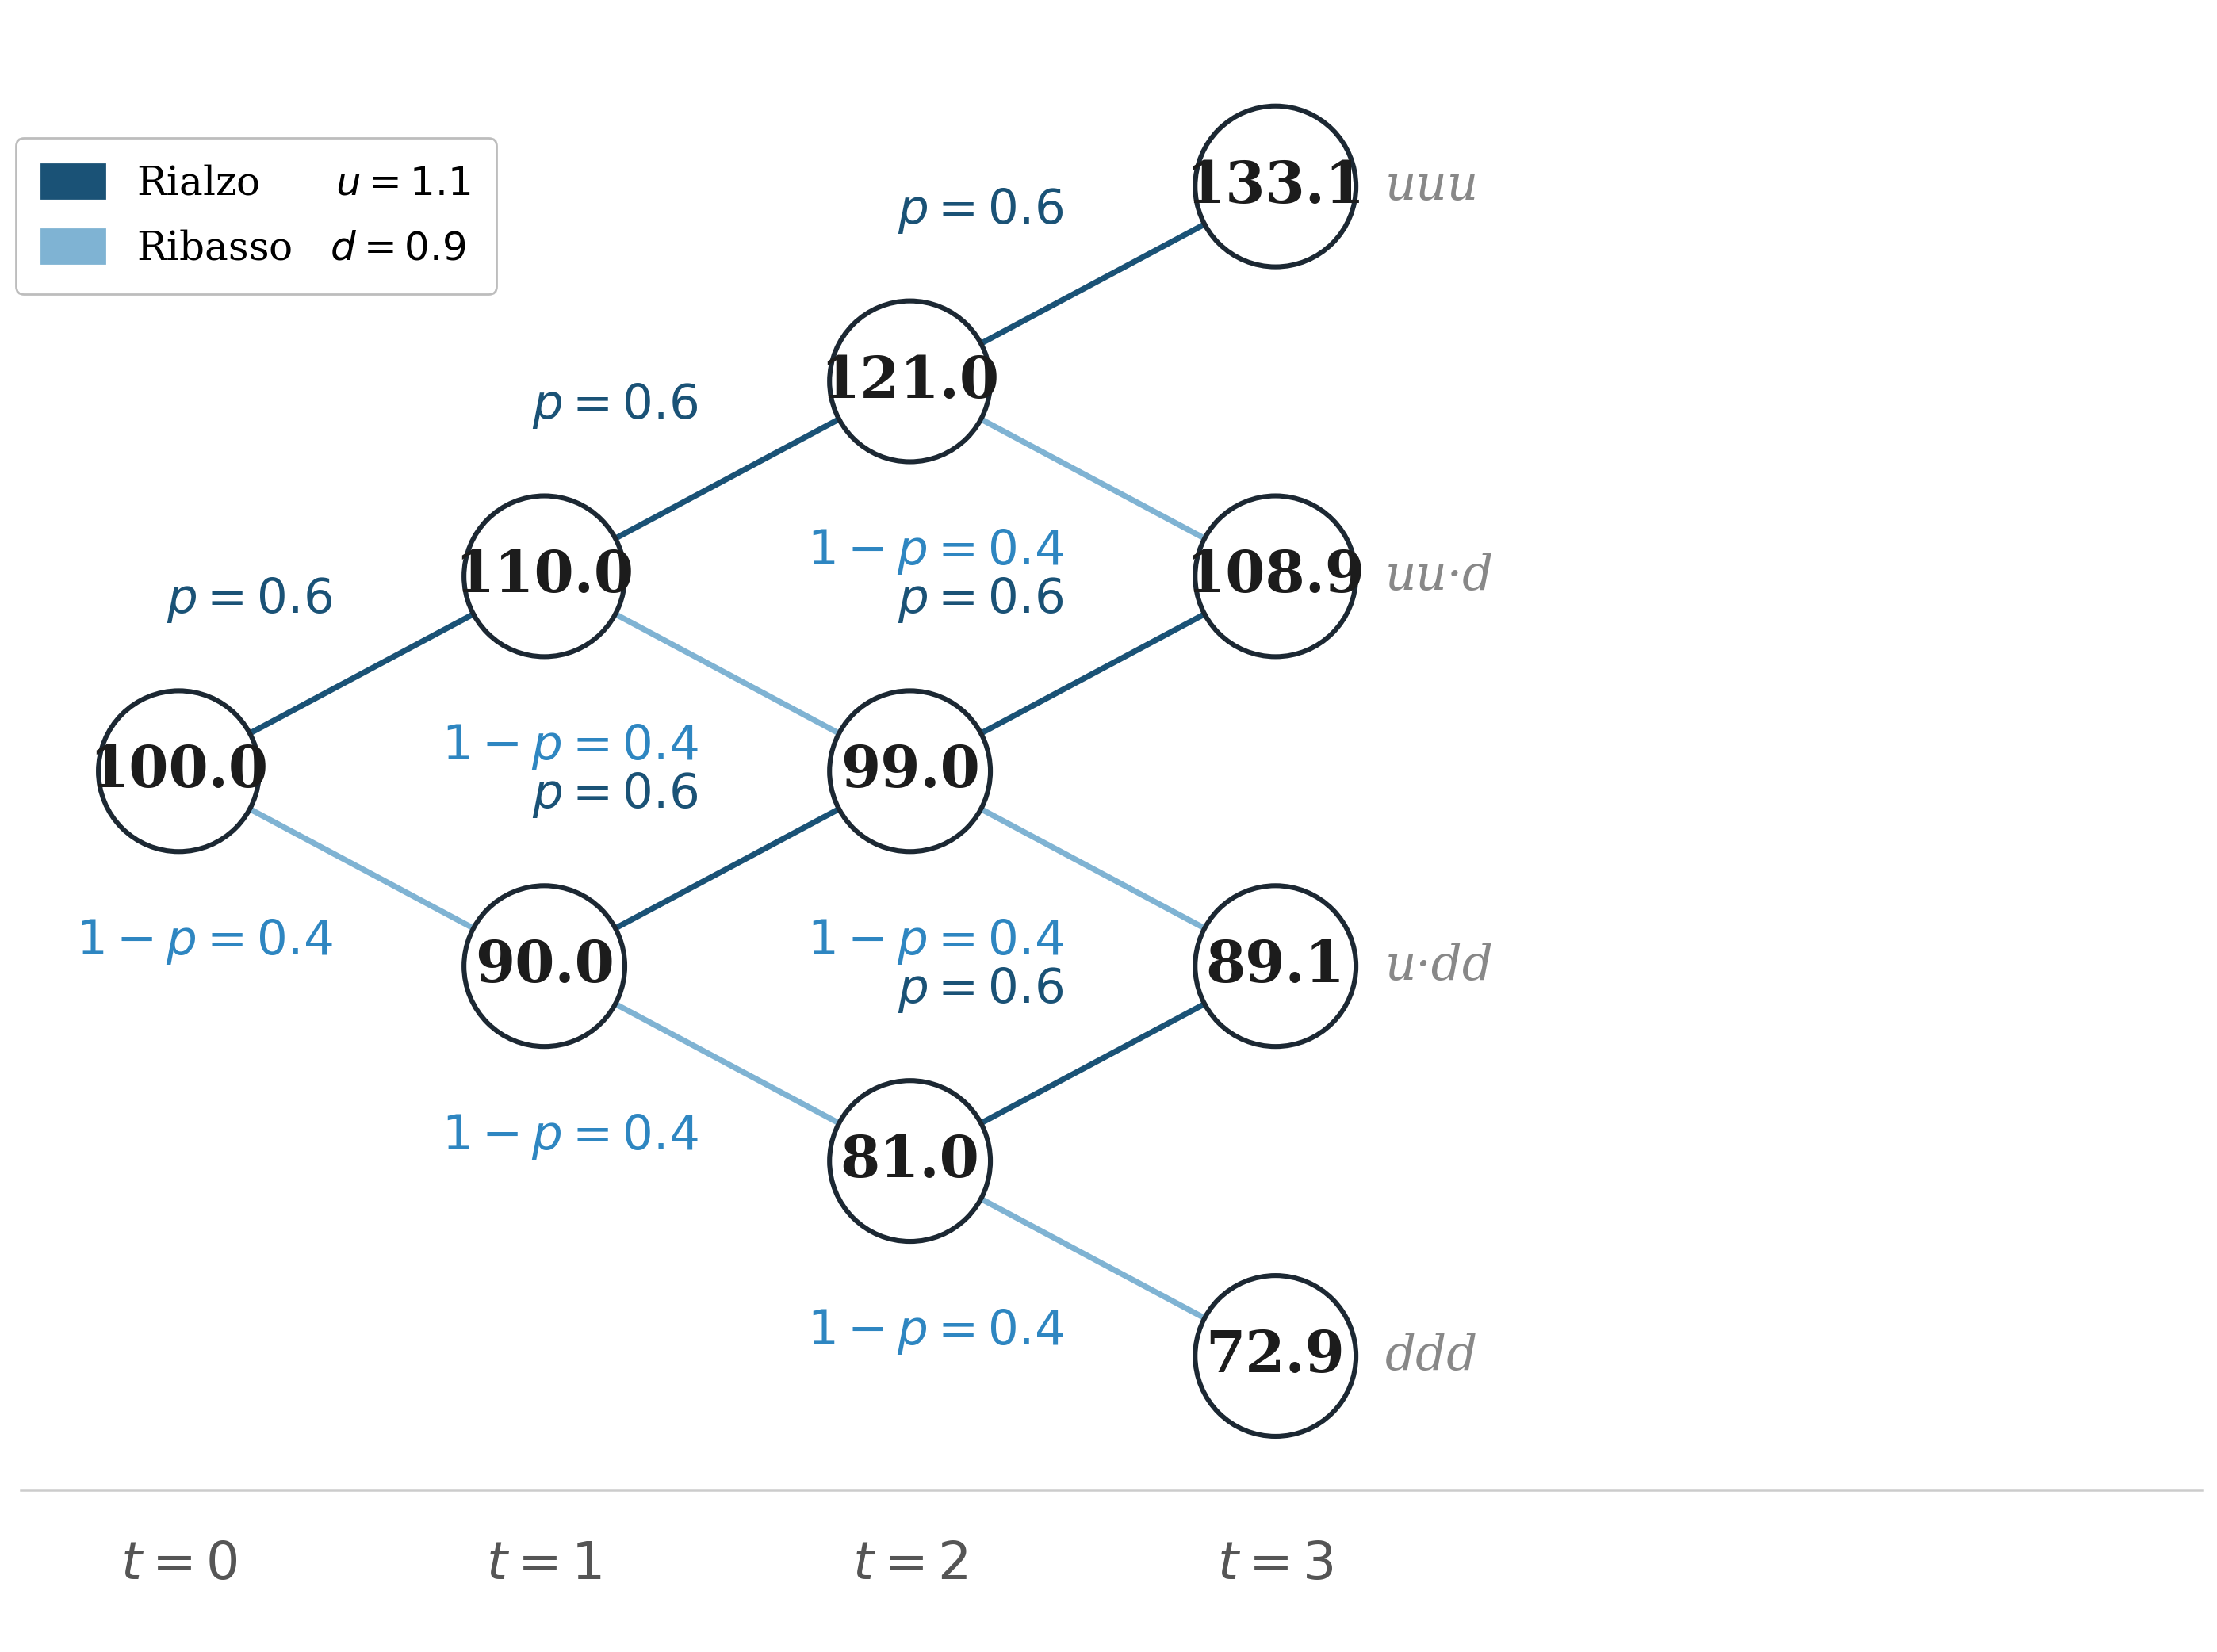
\includegraphics[width=0.92\textwidth]{../graphics/Cap04_Figura_4_1}
\caption{Albero binomiale dei prezzi con $S_0=100$, $u=1.1$,
$d=0.9$, $p=0.6$, $T=3$. Gli archi blu scuro indicano i movimenti
di rialzo (fattore $u$), gli archi azzurri quelli di ribasso
(fattore $d$). I nodi terminali corrispondono agli scenari
$s\in\mathcal{S}=\{1,\ldots,8\}$.}
\label{fig:albero-binomiale}
\end{figure}

La struttura ad albero rende visibili due propriet\`{a} fondamentali.
La prima \`{e} la \emph{non anticipativit\`{a}}: due traiettorie che
coincidono fino al tempo $t$ (cio\`{e} che passano per lo stesso nodo
al tempo $t$) non si distinguono sulla base dell'informazione $\F_t$.
La seconda \`{e} la \emph{ricombinazione}: nel modello binomiale,
poich\`{e} $ud=du$, traiettorie diverse che contengono lo stesso numero
di rialzi e ribassi raggiungono lo stesso nodo. Grazie a questa
propriet\`{a}, il numero di nodi distinti al tempo $t$ \`{e} $t+1$
anzich\`{e} $2^t$: i nodi crescono \emph{linearmente} con $t$, non
esponenzialmente. Per $T=3$ si hanno $4$ nodi terminali anzich\`{e}
$8$ traiettorie distinte, e il numero totale di nodi nell'albero \`{e}
$1+2+3+4=10$ anzich\`{e} $1+2+4+8=15$. Questa compressione \`{e}
computazionalmente cruciale: nei capitoli successivi consente di
calcolare prezzi e valori attesi condizionati su alberi con molti
passi in modo efficiente.

\begin{example}
\label{es:scenari-binomiale}
Per il modello con $S_0=100$, $u=1.1$, $d=0.9$, $p=0.6$, $T=3$, la
Tabella~\ref{tab:scenari-binomiale} elenca gli otto scenari con la
rispettiva probabilit\`{a} e il valore terminale.

\begin{table}[h]
\centering
\begin{tabular}{|c|c|c|c|}
\hline
\textbf{Scenario} $s$ & \textbf{Traiettoria} & $p_s$ & $S_3$\\
\hline
1 & $uuu$ & $0.216$ & $133.1$\\
2 & $uud$ & $0.144$ & $108.9$\\
3 & $udu$ & $0.144$ & $108.9$\\
4 & $duu$ & $0.144$ & $108.9$\\
5 & $udd$ & $0.096$ & $89.1$\\
6 & $dud$ & $0.096$ & $89.1$\\
7 & $ddu$ & $0.096$ & $89.1$\\
8 & $ddd$ & $0.064$ & $72.9$\\
\hline
\multicolumn{2}{|c|}{\textbf{Totale}} & $1.000$ & \\
\hline
\end{tabular}
\caption{Gli otto scenari del processo binomiale con $S_0=100$,
$u=1.1$, $d=0.9$, $p=0.6$, $T=3$.}
\label{tab:scenari-binomiale}
\end{table}
\end{example}


\begin{example}
\label{es:momenti-binomiale}
Per il processo binomiale con $S_0=100$, $u=1.1$, $d=0.9$, $p=0.6$,
$T=3$:
\[
m=0.6\cdot 1.1+0.4\cdot 0.9=1.02,
\qquad
m_2=0.6\cdot 1.21+0.4\cdot 0.81=1.050.
\]
I momenti del processo ai tre orizzonti sono riportati nella
Tabella~\ref{tab:momenti-binomiale}.

\begin{table}[h]
\centering
\begin{tabular}{|c|c|c|c|}
\hline
\textbf{Tempo} $t$ & $\mu(t)=\E[S_t]$ &
$\sigma^2(t)=\Var(S_t)$ & $\sigma(t)$\\
\hline
$0$ & $100.000$ & $0.000$ & $0.000$\\
$1$ & $102.000$ & $104.040$ & $10.200$\\
$2$ & $104.040$ & $215.523$ & $14.681$\\
$3$ & $106.121$ & $334.767$ & $18.297$\\
\hline
\end{tabular}
\caption{Media, varianza e deviazione standard del processo binomiale
($S_0=100$, $u=1.1$, $d=0.9$, $p=0.6$) ai tempi $t=0,1,2,3$. La
deviazione standard cresce con l'orizzonte: l'incertezza sul valore
futuro si accumula nel tempo, coerentemente con la struttura a
incrementi indipendenti.}
\label{tab:momenti-binomiale}
\end{table}

La covarianza tra $S_1$ e $S_3$ \`{e}:
\begin{eqnarray*}
\Cov(S_1,S_3)
&=& S_0^2\bigl(m_2^{\,1}\,m^{\,2}-m^{\,4}\bigr)\\
&=& 10000\,(1.050\cdot 1.0404-1.0824)\\
&=& 99.9,
\end{eqnarray*}
positiva, come atteso: prezzi elevati al tempo 1 tendono ad
accompagnarsi a prezzi elevati al tempo 3.
\end{example}



\subsection{L'incertezza cresce con l'orizzonte}

La Tabella~\ref{tab:momenti-binomiale} mostra che la deviazione
standard $\sigma(t)$ cresce al crescere di $t$. Questo fatto, che
nell'esempio \`{e} verificato numericamente, ha un significato
economico preciso: l'incertezza sul valore futuro di un'attivit\`{a}
finanziaria cresce con l'orizzonte di investimento.

\`{E} possibile quantificare questo effetto in modo esplicito. Per
il modello binomiale con incrementi i.i.d., si dimostra che la
deviazione standard cresce approssimativamente come $\sqrt{t}$ per
$t$ grande. Questo risultato \`{e} coerente con la propriet\`{a}
del moto browniano standard, per cui $\Var(W_t)=t$ e quindi
$\sigma(W_t)=\sqrt{t}$.

\begin{remark}
La crescita dell'incertezza con l'orizzonte ha implicazioni dirette
per la gestione del rischio. Il Value-at-Risk e il CVaR di una
posizione su un orizzonte di $T$ periodi non si ottengono
semplicemente moltiplicando per $T$ le misure di rischio a un
periodo: la struttura temporale della distribuzione delle perdite
deve essere modellata esplicitamente. Questo punto verr\`{a}
ripreso nel Capitolo~7.
\end{remark}


\subsection{Rendimenti logaritmici}

\noindent
\`{E} spesso conveniente descrivere il modello attraverso i
\emph{rendimenti logaritmici} anzich\`{e} i fattori moltiplicativi.
Si definisce
\[
r_t=\log\!\left(\frac{S_t}{S_{t-1}}\right)=\log R_t
\in\{\log u,\;\log d\}.
\]
Nel modello binomiale i rendimenti logaritmici $r_1,\ldots,r_T$ sono
indipendenti e identicamente distribuiti, con
\[
r_t=\begin{cases}
\log u & \text{con probabilit\`{a} }p,\\
\log d & \text{con probabilit\`{a} }1-p.
\end{cases}
\]
Il prezzo si scrive allora come esponenziale di una somma di
rendimenti logaritmici i.i.d.:
\[
S_t=S_0\exp\!\left(\sum_{k=1}^{t}r_k\right).
\]
Il logaritmo del prezzo, $\log S_t=\log S_0+\sum_{k=1}^{t}r_k$,
\`{e} dunque una passeggiata aleatoria nel senso
dell'Esempio~\ref{es:random-walk}. Questa osservazione anticipa il
legame tra il modello binomiale e il moto browniano geometrico: nel
Capitolo~6 vedremo che, facendo tendere a zero l'ampiezza del passo
temporale, la passeggiata aleatoria dei rendimenti logaritmici
converge a un moto browniano, e il modello binomiale dei prezzi al
corrispondente moto browniano geometrico.

\subsection{Sigma-algebra generata da una variabile casuale
e partizione di $\Omega$}

\noindent
Nel Capitolo~3 la sigma-algebra generata da una partizione
$\{B_1,\ldots,B_n\}$ di $\Omega$ era definita come l'insieme di tutti
gli eventi ottenibili come unioni dei blocchi $B_i$. Nella
Sezione~\ref{sec:momenti2} abbiamo introdotto la notazione
$\sigma(X_0,X_1,\ldots,X_t)$: la sigma-algebra \emph{generata da
variabili casuali}. Nel caso del modello binomiale \`{e} importante
verificare esplicitamente che le due notazioni descrivono lo stesso
oggetto, rendendo concreto e calcolabile il concetto generale.

La sigma-algebra $\sigma(X)$ generata da una variabile casuale $X$
che assume un numero finito di valori $v_1,\ldots,v_k$ coincide con
la sigma-algebra generata dalla partizione
\[
\bigl\{\{X=v_1\},\;\ldots,\;\{X=v_k\}\bigr\}.
\]
Conoscere il valore di $X$ equivale dunque a sapere in quale blocco
della partizione si trova l'esito $\omega$. La
Tabella~\ref{tab:sigma-partizione} mostra esplicitamente questa
corrispondenza per la filtrazione naturale del modello binomiale.

\begin{table}[h]
\centering
\begin{tabular}{|p{1.2cm}|p{3.5cm}|p{6.0cm}|}
\hline
\textbf{Tempo} $t$ & \textbf{Sigma-algebra} & \textbf{Partizione
corrispondente di $\Omega$}\\
\hline
$t=0$ & $\F_0=\sigma(S_0)=\{\emptyset,\Omega\}$ &
Unico blocco: \newline $\{uuu,uud,udu,udd,duu,dud,ddu,ddd\}$\\
\hline
$t=1$ & $\F_1=\sigma(S_1)$ &
Due blocchi: \newline $A_u=\{uuu,uud,udu,udd\}$ e \newline
$A_d=\{duu,dud,ddu,ddd\}$\\
\hline
$t=2$ & $\F_2=\sigma(S_1,S_2)$ &
Quattro blocchi: $A_{uu}=\{uuu,uud\}$,
$A_{ud}=\{udu,udd\}$,
$A_{du}=\{duu,dud\}$,
$A_{dd}=\{ddu,ddd\}$\\
\hline
$t=3$ & $\F_3=\sigma(S_1,S_2,S_3)$ &
Otto blocchi: ogni esito elementare forma un blocco
da solo, ad esempio $\{uuu\}$, $\{uud\}$, \ldots,
$\{ddd\}$\\
\hline
\end{tabular}
\caption{Sigma-algebre della filtrazione naturale del processo
binomiale ($S_0=100$, $u=1.1$, $d=0.9$, $T=3$) e partizioni
corrispondenti di $\Omega$. Ogni riga mostra come l'informazione
disponibile al tempo $t$ si traduca in una suddivisione di
$\Omega$ in blocchi indistinguibili sulla base delle osservazioni
fino a $t$.}
\label{tab:sigma-partizione}
\end{table}

\noindent
La tabella chiarisce che la notazione $\sigma(S_1,\ldots,S_t)$ non
aggiunge complessit\`{a} rispetto a quella del Capitolo~3: indica
semplicemente la sigma-algebra generata dalla partizione indotta dai
valori osservati del processo fino al tempo $t$.

\subsection{Filtrazione naturale e processo delle previsioni}

\noindent
La definizione generale di filtrazione naturale \`{e} stata introdotta
nella Sezione~\ref{sec:momenti2}. Nel modello binomiale essa ha una
struttura particolarmente trasparente: al tempo $t=0$ l'unica
informazione disponibile \`{e} quella banale, $\F_0=\{\emptyset,
\Omega\}$; al tempo $t=1$ si sa se il primo movimento \`{e} stato $u$
o $d$, e $\F_1$ distingue i due blocchi $A_u$ e $A_d$; al tempo $t=2$
si conoscono i primi due movimenti e $\F_2$ distingue quattro blocchi;
al tempo $t=3$ l'intera traiettoria \`{e} nota e $\F_3$ distingue
tutti e otto gli esiti.

Su questa filtrazione possiamo costruire concretamente il processo
delle previsioni introdotto in astratto nella
Sezione~\ref{sec:martingale}: la previsione del prezzo terminale
$S_3$ aggiornata all'informazione disponibile a ogni istante.

\begin{example}
\label{es:filtrazione-binomiale}
Nel processo binomiale con $S_0=100$, $u=1.1$, $d=0.9$, $p=0.6$,
$T=3$, calcoliamo il processo delle previsioni
$H_t=\E[S_3\mid\F_t]$ per $t=0,1,2,3$.

\paragraph{Una formula compatta.}
Poich\`{e} $S_3=S_t\cdot R_{t+1}\cdots R_3$ e i fattori futuri sono
indipendenti dall'informazione $\F_t$, con $\E[R_k]=m=1.02$:
\[
H_t=\E[S_3\mid\F_t]
=S_t\,\E[R_{t+1}\cdots R_3\mid\F_t]
=S_t\,m^{\,3-t}.
\]
La previsione del prezzo terminale \`{e} dunque il prezzo corrente
$S_t$ capitalizzato al rendimento medio $m$ per i periodi residui.

\paragraph{Calcolo nei due nodi al tempo $t=1$.}
Al tempo $t=1$ la filtrazione distingue il nodo $A_u$ (prezzo corrente
$S_1=110$) e il nodo $A_d$ ($S_1=90$). Verifichiamo la formula
compatta tramite il calcolo diretto. Per $\omega\in A_u$ i tre valori
terminali raggiungibili sono
\[
S_3=\begin{cases}
u^2\cdot 110=133.1 & \text{con probabilit\`{a} }p^2=0.36,\\
ud\cdot 110=108.9 & \text{con probabilit\`{a} }2p(1-p)=0.48,\\
d^2\cdot 110=89.1 & \text{con probabilit\`{a} }(1-p)^2=0.16,
\end{cases}
\]
da cui
\[
\E[S_3\mid A_u]=133.1\cdot 0.36+108.9\cdot 0.48+89.1\cdot 0.16
=114.444,
\]
in accordo con $S_1\,m^2=110\cdot 1.0404=114.444$. Analogamente, per
$\omega\in A_d$:
\[
\E[S_3\mid A_d]=108.9\cdot 0.36+89.1\cdot 0.48+72.9\cdot 0.16
=93.636=90\cdot 1.0404.
\]

\paragraph{Il processo delle previsioni sull'albero.}
Applicando la formula $H_t=S_t\,m^{\,3-t}$ a tutti i nodi si ottiene
il processo delle previsioni completo, riportato nella
Tabella~\ref{tab:previsioni-binomiale}.

\begin{table}[h]
\centering
\begin{tabular}{|c|l|}
\hline
\textbf{Tempo} $t$ & \textbf{Valori di } $H_t=\E[S_3\mid\F_t]$
\textbf{ nei nodi}\\
\hline
$0$ & $106.121$\\
$1$ & $114.444$ (nodo $u$), \quad $93.636$ (nodo $d$)\\
$2$ & $123.420$ (uu), \quad $100.980$ (ud), \quad $82.620$ (dd)\\
$3$ & $133.100$ (uuu), \quad $108.900$ (uud), \quad
       $89.100$ (udd), \quad $72.900$ (ddd)\\
\hline
\end{tabular}
\caption{Il processo delle previsioni $H_t=\E[S_3\mid\F_t]=S_t\,
m^{\,3-t}$ in tutti i nodi dell'albero binomiale. Al tempo $t=3$ la
previsione coincide con il valore realizzato $S_3$; al tempo $t=0$
coincide con la media incondizionata $\E[S_3]=106.121$.}
\label{tab:previsioni-binomiale}
\end{table}

\paragraph{Il processo delle previsioni \`{e} una martingala.}
Il processo $\{H_t\}$ \`{e} una martingala rispetto a $\{\F_t\}$, in
accordo con il risultato generale sulla martingala di Doob
(Sezione~\ref{sec:martingale}). Verifichiamolo su un passo, dal nodo
$u$ al tempo $1$ ai suoi due successori al tempo $2$ (i nodi uu e ud):
\[
\E[H_2\mid A_u]=0.6\cdot 123.420+0.4\cdot 100.980
=74.052+40.392=114.444=H_1(A_u).
\]
La previsione fatta oggi della previsione di domani coincide con la
previsione di oggi: le revisioni della previsione non sono prevedibili
in anticipo. In particolare, prendendo il valore atteso dal tempo $1$
al tempo $0$ si ritrova la propriet\`{a} della torre:
\[
\E[H_1]=0.6\cdot 114.444+0.4\cdot 93.636=106.121=\E[S_3].
\]

\paragraph{Attenzione: il processo dei prezzi non \`{e} una
martingala.} \`{E} importante non confondere il processo delle
previsioni $\{H_t\}$ con il processo dei prezzi $\{S_t\}$. Il primo
\`{e} sempre una martingala. Il secondo lo \`{e} solo se il rendimento
medio per periodo \`{e} unitario, $m=1$. Nel nostro esempio $m=1.02>1$,
e infatti
\[
\E[S_1\mid\F_0]=0.6\cdot 110+0.4\cdot 90=102=S_0\,m>S_0:
\]
il processo dei prezzi \`{e} una submartingala, coerentemente con il
fatto che un investimento azionario ha rendimento atteso positivo. La
condizione $m=1$, sotto la quale il prezzo diventa una martingala, ha
un ruolo centrale nella valutazione risk-neutral, che riprenderemo nei
capitoli dedicati al pricing.
\end{example}

% ============================================================
% MQF_Cap_05_Sezione_5_7.tex
% Capitolo 5 - Sezione 5.7
% Simulazione: logica generale e stima Monte Carlo
%
% Sezione nuova. Resta a livello generale (tempo discreto):
% niente modelli continui specifici ne' Eulero-Maruyama,
% che arrivano nel Capitolo 6.
% ============================================================

\section{Simulazione: logica generale e stima Monte Carlo}
\label{sec:simulazione}

\noindent
Molte quantit\`{a} di interesse in finanza --- il prezzo atteso di un
contratto, la perdita attesa di un portafoglio, la probabilit\`{a} di
superare una soglia di rischio --- si esprimono come valori attesi di
funzioni di un processo stocastico. In casi semplici, come il modello
binomiale della Sezione~\ref{sec:binomiale}, questi valori attesi si
calcolano in forma chiusa sommando su tutti gli scenari. Ma non appena
il numero di periodi cresce, o la dinamica del processo si fa pi\`{u}
complessa, l'enumerazione esplicita di tutti gli scenari diventa
impraticabile: un albero binomiale con $T=50$ periodi ha gi\`{a}
$2^{50}$ traiettorie, oltre mille miliardi. In questi casi si ricorre
alla \emph{simulazione}.

L'idea della simulazione \`{e} semplice e potente: invece di enumerare
tutti gli scenari possibili, se ne generano molti \emph{a caso},
coerentemente con la legge del processo, e si stima la quantit\`{a} di
interesse come media empirica sui soli scenari generati. Questa
sezione ne presenta la logica in forma generale, valida per qualunque
processo a tempo discreto. La sua applicazione ai modelli in tempo
continuo, mediante la discretizzazione delle equazioni differenziali
stocastiche, sar\`{a} sviluppata nel Capitolo~6 e implementata in
Python nella lezione applicativa.

\subsection{Generazione di traiettorie}

\noindent
Simulare un processo $\{X_t\}_{t=0}^{T}$ significa generare una
\emph{replica} della sua traiettoria, ovvero una sequenza di valori
$X_0^{(k)},X_1^{(k)},\ldots,X_T^{(k)}$ che costituisce una possibile
realizzazione del processo. Generando $M$ repliche indipendenti
\[
\bigl\{X_0^{(k)},X_1^{(k)},\ldots,X_T^{(k)}\bigr\},
\qquad k=1,2,\ldots,M,
\]
si ottiene un campione di $M$ traiettorie, ciascuna corrispondente a
un possibile percorso del processo.

Per un processo definito da una dinamica ricorsiva --- come il modello
binomiale, in cui $X_{t+1}$ si ottiene da $X_t$ applicando un
movimento aleatorio --- la generazione di una traiettoria procede in
modo sequenziale: si parte dal valore iniziale $X_0$, noto, e a ogni
passo si estrae l'innovazione casuale (nel caso binomiale, il
movimento $u$ o $d$) e si calcola il valore successivo. Ripetendo la
procedura per $T$ passi si ottiene un'intera traiettoria; ripetendola
per $M$ repliche indipendenti si ottiene il campione.

\begin{remark}
La fedelt\`{a} della simulazione dipende interamente dalla qualit\`{a}
del generatore di numeri casuali utilizzato per estrarre le
innovazioni. I generatori impiegati nella pratica sono in realt\`{a}
\emph{pseudo-casuali}: producono sequenze deterministiche che
imitano le propriet\`{a} statistiche dell'aleatoriet\`{a}. Questo ha
un risvolto utile: fissando il \emph{seme} (seed) del generatore, una
simulazione diventa esattamente riproducibile, il che \`{e}
essenziale per il controllo e la validazione dei risultati. Questo
aspetto operativo sar\`{a} ripreso nella lezione in Python.
\end{remark}

\subsection{La stima Monte Carlo}

\noindent
Supponiamo di voler calcolare il valore atteso $\E[g(X_T)]$ di una
funzione del processo --- ad esempio $g(X_T)=X_T$ per il valore atteso
terminale, oppure $g(X_T)=\max(X_T-K,0)$ per il payoff di un'opzione
call con prezzo di esercizio $K$. La \emph{stima Monte Carlo} di
questo valore atteso \`{e} la media empirica della funzione sulle $M$
traiettorie simulate:
\[
\widehat{\theta}_M=\frac{1}{M}\sum_{k=1}^{M}g\bigl(X_T^{(k)}\bigr).
\]
La giustificazione teorica di questa stima \`{e} la legge dei grandi
numeri, gi\`{a} incontrata nel Capitolo~2: poich\`{e} le repliche sono
indipendenti e identicamente distribuite, la media empirica converge
al valore atteso vero al crescere del numero di repliche,
\[
\widehat{\theta}_M\xrightarrow[M\to\infty]{}\theta=\E[g(X_T)].
\]
La simulazione Monte Carlo trasforma dunque il calcolo di un valore
atteso --- operazione che richiederebbe la conoscenza dell'intera
distribuzione di $g(X_T)$ --- in un semplice problema di media
campionaria, al prezzo di un errore di stima che, come vedremo,
si pu\`{o} controllare.

La stessa logica si applica a quantit\`{a} condizionate. La media di
$g(X_T)$ ristretta agli scenari che soddisfano una certa condizione
$A$ --- ad esempio gli scenari in cui il processo non scende mai sotto
una soglia --- si stima con
\[
\widehat{\theta}_M^{\,A}
=\frac{1}{M_A}\sum_{k:\,\omega^{(k)}\in A}g\bigl(X_T^{(k)}\bigr),
\qquad
M_A=\#\{k:\omega^{(k)}\in A\},
\]
ovvero come media della funzione sui soli scenari che ricadono in $A$,
dove $M_A$ \`{e} il numero di tali scenari.

\begin{example}[Stima del prezzo atteso terminale]
\label{es:montecarlo-binomiale}
Si consideri il modello binomiale con $S_0=100$, $u=1.1$, $d=0.9$,
$p=0.6$, $T=3$. Il valore atteso terminale esatto, calcolato nella
Sezione~\ref{sec:binomiale}, \`{e} $\E[S_3]=106.121$. Una simulazione
Monte Carlo lo stima generando $M$ traiettorie e mediando i valori
terminali $S_3^{(k)}$. Al crescere di $M$, la stima
$\widehat{\theta}_M$ si avvicina al valore esatto: con poche centinaia
di repliche l'approssimazione \`{e} gi\`{a} ragionevole, con alcune
decine di migliaia diventa accurata alle prime cifre decimali. In un
modello cos\`{\i} semplice la simulazione non \`{e} necessaria, poich\`{e}
il valore esatto \`{e} noto; ma essa fornisce un banco di prova ideale,
perch\`{e} permette di confrontare la stima simulata con il risultato
analitico e di verificare cos\`{\i} la correttezza della procedura ---
un passo di validazione che riprenderemo in Python.
\end{example}

\subsection{L'incertezza della stima}

\noindent
La stima Monte Carlo \`{e} essa stessa una quantit\`{a} aleatoria:
ripetendo l'intera simulazione con un diverso insieme di numeri
casuali si otterrebbe un valore leggermente diverso. \`{E} dunque
essenziale accompagnare la stima con una misura della sua incertezza.

Indichiamo con $\sigma_g^2=\Var\bigl(g(X_T)\bigr)$ la varianza della
quantit\`{a} simulata su una singola replica. Poich\`{e} la stima
$\widehat{\theta}_M$ \`{e} la media di $M$ repliche indipendenti, la
sua varianza \`{e}
\[
\Var\bigl(\widehat{\theta}_M\bigr)=\frac{\sigma_g^2}{M},
\]
e la sua deviazione standard --- detta \emph{errore standard} della
stima --- \`{e}
\[
\operatorname{SE}\bigl(\widehat{\theta}_M\bigr)
=\frac{\sigma_g}{\sqrt{M}}.
\]
Nella pratica $\sigma_g$ non \`{e} noto e si stima a sua volta dalla
deviazione standard campionaria delle repliche.

Questa formula racchiude la propriet\`{a} fondamentale --- e il limite
principale --- del metodo Monte Carlo: l'errore di stima decresce come
$1/\sqrt{M}$. Per dimezzare l'errore standard occorre quadruplicare il
numero di repliche; per guadagnare una cifra decimale di precisione
occorre moltiplicare per cento il numero di simulazioni. Questa
convergenza lenta \`{e} il prezzo della generalit\`{a} del metodo, ed
\`{e} la ragione per cui esistono numerose tecniche di
\emph{riduzione della varianza}, volte a diminuire $\sigma_g$ a
parit\`{a} di $M$, che la lezione in Python avr\`{a} modo di
illustrare.

\begin{remark}
Il fatto che l'errore decresca come $1/\sqrt{M}$, indipendentemente
dal numero di periodi $T$ o dalla complessit\`{a} del processo, \`{e}
ci\`{o} che rende la simulazione Monte Carlo cos\`{\i} preziosa nelle
applicazioni finanziarie. Mentre l'enumerazione esplicita degli
scenari ha un costo che cresce esponenzialmente con $T$, il costo
della simulazione cresce solo linearmente con $M$ e con $T$. \`{E}
per questo che la simulazione diventa il metodo di elezione non
appena la dimensione del problema supera la soglia in cui i metodi
esatti restano praticabili --- una situazione tipica nei modelli in
tempo continuo del prossimo capitolo, dove ogni traiettoria \`{e}
ottenuta discretizzando un'equazione differenziale stocastica su una
griglia temporale fitta.
\end{remark}

% ============================================================
% MQF_Cap_05_Sezione_5_8.tex
% Capitolo 5 - Sezione 5.8
% Esercizi svolti
%
% Formato soluzioni: \textbf{Soluzione.} + itemize
% (non si usa l'ambiente solution)
% ============================================================

\section{Esercizi svolti}
\label{sec:esercizi-svolti}

\begin{exercise}[Profitto cumulato di un desk di trading]
\label{ex:random-walk}
Un desk di trading realizza ogni giorno un profitto $Z_k$ che,
in migliaia di euro, assume due valori:
\[
Z_k=\begin{cases}
+3 & \text{con probabilit\`{a} }0.5,\\
-1 & \text{con probabilit\`{a} }0.5,
\end{cases}
\]
con i diversi giorni indipendenti e identicamente distribuiti. Il
profitto cumulato dopo $t$ giorni \`{e} $X_t=\sum_{k=1}^{t}Z_k$, con
$X_0=0$.
\begin{enumerate}
\item Calcolare media e varianza del profitto giornaliero (uguali per
ogni giorno, essendo le $Z_k$ i.i.d.).
\item Determinare le funzioni $\mu(t)=\E[X_t]$ e
$\sigma^2(t)=\Var(X_t)$.
\item Calcolare $\Cov(X_2,X_5)$.
\item Stabilire se $\{X_t\}$ \`{e} una martingala, una submartingala
o una supermartingala rispetto alla propria filtrazione naturale.
\end{enumerate}
\end{exercise}

\noindent
\textbf{Soluzione.}
\begin{enumerate}
\item Poich\'{e} le variabili $Z_1,Z_2,\ldots$ sono identicamente
distribuite, media e varianza non dipendono dall'indice: il calcolo
svolto per un generico tempo $k$ vale per ogni giorno. Per ogni
$k\geq 1$,
\[
\nu=\E[Z_k]=0.5\cdot 3+0.5\cdot(-1)=1.
\]
Per la varianza, sempre per ogni $k\geq 1$,
\[
\E[Z_k^2]=0.5\cdot 9+0.5\cdot 1=5,
\qquad
\tau^2=\Var(Z_k)=\E[Z_k^2]-\nu^2=5-1=4.
\]

\item Trattandosi di una passeggiata aleatoria con incrementi
i.i.d., per i risultati della Sezione~\ref{sec:momenti2}:
\[
\mu(t)=t\,\nu=t,
\qquad
\sigma^2(t)=t\,\tau^2=4t.
\]
La deviazione standard $\sigma(t)=2\sqrt{t}$ cresce con la radice
dell'orizzonte: l'incertezza sul profitto cumulato si accumula nel
tempo.

\item Per la struttura di covarianza della passeggiata aleatoria, con
$s\leq t$ vale $c(s,t)=\min(s,t)\,\tau^2$. Quindi
\[
\Cov(X_2,X_5)=\min(2,5)\cdot 4=2\cdot 4=8.
\]

\item Per $s\leq t$:
\[
\E[X_t\mid\F_s]=X_s+(t-s)\,\nu=X_s+(t-s)\geq X_s,
\]
con disuguaglianza stretta per $t>s$. Il processo \`{e} dunque una
\emph{submartingala}: il desk ha un vantaggio sistematico
($\nu=1>0$), e il profitto cumulato tende a crescere in media. Solo
se il profitto medio giornaliero fosse nullo il processo sarebbe una
martingala.
\end{enumerate}

\begin{exercise}[Albero binomiale a due periodi]
\label{ex:binomiale}
Un'azione vale oggi $S_0=80$. A ogni periodo il prezzo sale del
$25\%$ (fattore $u=1.25$) con probabilit\`{a} $p=0.5$, oppure scende
del $20\%$ (fattore $d=0.8$) con probabilit\`{a} $1-p=0.5$. Si
considera l'orizzonte $T=2$.
\begin{enumerate}
\item Costruire l'albero dei prezzi ed elencare gli scenari con le
rispettive probabilit\`{a}.
\item Calcolare $\E[S_2]$ e verificarlo con la formula
$\E[S_2]=S_0\,m^2$.
\item Calcolare $\E[S_2\mid\F_1]$ nei due nodi al tempo $1$ e
verificare la propriet\`{a} della torre.
\end{enumerate}
\end{exercise}

\noindent
\textbf{Soluzione.}
\begin{enumerate}

\item Il rendimento lordo medio per periodo \`{e}
\[
m=pu+(1-p)d=0.5\cdot 1.25+0.5\cdot 0.8=1.025.
\]
I valori del prezzo nei nodi sono:
\[
\begin{array}{ll}
t=0: & S_0=80;\\
t=1: & S_1^u=80\cdot 1.25=100, \quad S_1^d=80\cdot 0.8=64;\\
t=2: & S_2^{uu}=125, \quad S_2^{ud}=S_2^{du}=80,
       \quad S_2^{dd}=51.2.
\end{array}
\]
I quattro scenari, con probabilit\`{a} $p_s=0.25$ ciascuno (essendo
$p=0.5$), sono: $uu$ con $S_2=125$; $ud$ e $du$ con $S_2=80$; $dd$ con
$S_2=51.2$.

\item Sommando sugli scenari:
\[
\E[S_2]=0.25\cdot 125+0.5\cdot 80+0.25\cdot 51.2
=31.25+40+12.8=84.05.
\]
La formula compatta conferma: $\E[S_2]=S_0\,m^2=80\cdot
1.025^2=80\cdot 1.050625=84.05$.

\item Al nodo $u$ ($S_1=100$), i due esiti al tempo $2$ sono $125$ e
$80$, ciascuno con probabilit\`{a} $0.5$:
\[
\E[S_2\mid A_u]=0.5\cdot 125+0.5\cdot 80=102.5=100\cdot 1.025.
\]
Al nodo $d$ ($S_1=64$), gli esiti sono $80$ e $51.2$:
\[
\E[S_2\mid A_d]=0.5\cdot 80+0.5\cdot 51.2=65.6=64\cdot 1.025.
\]
Verifica della torre:
\[
\E\bigl[\E[S_2\mid\F_1]\bigr]
=0.5\cdot 102.5+0.5\cdot 65.6=51.25+32.8=84.05=\E[S_2].
\]
\end{enumerate}

\begin{exercise}[Prezzo scontato e misura di martingala]
\label{ex:scontato}
Si consideri un periodo singolo. Un'azione vale $S_0=100$ e tra un
periodo varr\`{a} $S_1=120$ (rialzo) oppure $S_1=90$ (ribasso). Il
tasso privo di rischio per il periodo \`{e} $r=0.05$. Si definisca la
probabilit\`{a} di rialzo $q$ in modo che il prezzo scontato
$\tilde{S}_t=S_t/(1+r)^t$ sia una martingala, cio\`{e} tale che
$\E_{\Q}[\tilde{S}_1]=\tilde{S}_0=S_0$.
\begin{enumerate}
\item Determinare il valore di $q$.
\item Verificare che, sotto tale probabilit\`{a}, il prezzo scontato
soddisfa la propriet\`{a} di martingala.
\item Interpretare il risultato.
\end{enumerate}
\end{exercise}

\noindent
\textbf{Soluzione.}
\begin{enumerate}
\item La condizione di martingala per il prezzo scontato su un periodo
\`{e}
\[
\frac{1}{1+r}\,\E_{\Q}[S_1]=S_0,
\qquad\text{ossia}\qquad
\E_{\Q}[S_1]=S_0(1+r).
\]
Con $\E_{\Q}[S_1]=q\cdot 120+(1-q)\cdot 90$ e $S_0(1+r)=105$:
\[
120q+90(1-q)=105
\;\Longrightarrow\;
30q=15
\;\Longrightarrow\;
q=0.5.
\]
In generale $q=\dfrac{(1+r)S_0-S_1^d}{S_1^u-S_1^d}
=\dfrac{105-90}{120-90}=0.5$, formula che riprenderemo nei capitoli
sul pricing.

\item Sotto $\Q$ con $q=0.5$:
\[
\E_{\Q}[\tilde{S}_1]
=\frac{1}{1.05}\bigl(0.5\cdot 120+0.5\cdot 90\bigr)
=\frac{105}{1.05}=100=\tilde{S}_0.
\]
Il prezzo scontato \`{e} dunque una martingala sotto $\Q$.

\item La probabilit\`{a} $q=0.5$ non \`{e} la probabilit\`{a}
\emph{fisica} con cui il mercato sale o scende, ma una probabilit\`{a}
\emph{artificiale} --- la misura risk-neutral $\Q$ --- costruita in
modo che il prezzo scontato dell'azione diventi una martingala. Sotto
questa misura, ogni attivit\`{a} ha rendimento atteso pari al tasso
privo di rischio. \`{E} questa la propriet\`{a} che, nei capitoli sul
pricing, consentir\`{a} di valutare un derivato come valore atteso
scontato del suo payoff sotto $\Q$.
\end{enumerate}

\begin{exercise}[Dimensionamento di una simulazione Monte Carlo]
\label{ex:montecarlo}
Si vuole stimare per simulazione il prezzo atteso $\theta=\E[g(X_T)]$
di un contratto. Una simulazione pilota con $M_0=1\,000$ repliche
fornisce una stima $\widehat{\theta}=12.4$ e una deviazione standard
campionaria delle repliche pari a $s_g=15$.
\begin{enumerate}
\item Stimare l'errore standard della stima pilota e costruire un
intervallo di confidenza approssimato al $95\%$ per $\theta$.
\item Determinare il numero di repliche necessario affinch\'{e}
l'errore standard scenda a $0.05$.
\end{enumerate}
\end{exercise}

\noindent
\textbf{Soluzione.}
\begin{enumerate}
\item L'errore standard della stima pilota \`{e}
\[
\operatorname{SE}=\frac{s_g}{\sqrt{M_0}}
=\frac{15}{\sqrt{1\,000}}
=\frac{15}{31.62}\approx 0.474.
\]
Un intervallo di confidenza approssimato al $95\%$, usando il
quantile $1.96$ della normale standard, \`{e}
\[
\widehat{\theta}\pm 1.96\cdot\operatorname{SE}
=12.4\pm 1.96\cdot 0.474
=12.4\pm 0.93,
\]
ossia all'incirca l'intervallo $[11.47,\;13.33]$.

\item Imponendo $\operatorname{SE}=s_g/\sqrt{M}\leq 0.05$ e
risolvendo per $M$:
\[
\sqrt{M}\geq\frac{s_g}{0.05}=\frac{15}{0.05}=300
\;\Longrightarrow\;
M\geq 300^2=90\,000.
\]
Per ridurre l'errore standard da $0.474$ a $0.05$, ovvero di un
fattore circa $9.5$, occorre aumentare il numero di repliche di un
fattore $9.5^2\approx 90$: dalle mille repliche iniziali a circa
novantamila. Questo illustra concretamente la convergenza $1/\sqrt{M}$
del metodo Monte Carlo, e il motivo per cui, quando l'accuratezza
richiesta \`{e} elevata, diventano interessanti le tecniche di
riduzione della varianza.
\end{enumerate}

% ============================================================
% MQF_Cap_05_Sezione_5_9.tex
% Capitolo 5 - Sezione 5.9
% Esercizi proposti
%
% Sei esercizi di difficolta' crescente. Per ciascuno e' indicato
% il solo risultato finale, per l'autovalutazione (puo' essere
% rimosso se si preferisce non fornirlo).
% ============================================================

\section{Esercizi proposti}
\label{sec:esercizi-proposti}

\begin{exercise}[Posizione di cassa aleatoria]
\label{ex:prop-rw}
La posizione di cassa giornaliera di un'attivit\`{a} varia ogni giorno
di una quantit\`{a} $Z_k$ che vale $+2$ con probabilit\`{a} $0.6$ e
$-2$ con probabilit\`{a} $0.4$ (in migliaia di euro), con giorni
indipendenti. Sia $X_t=\sum_{k=1}^{t}Z_k$ la posizione cumulata,
$X_0=0$.
\begin{enumerate}
\item Calcolare media e varianza di $Z_k$.
\item Determinare $\mu(t)$ e $\sigma(t)$, e calcolare i loro valori
per $t=10$.
\item Stabilire se $\{X_t\}$ \`{e} martingala, submartingala o
supermartingala.
\end{enumerate}
\textit{Risultati:} $\nu=0.4$, $\tau^2=3.84$; $\mu(10)=4$,
$\sigma(10)\approx 6.20$; submartingala.
\end{exercise}

\begin{exercise}[Albero binomiale a tre periodi]
\label{ex:prop-binomiale}
Un'azione vale $S_0=50$. A ogni periodo sale del $20\%$ ($u=1.2$) con
probabilit\`{a} $p=0.55$, oppure scende del $10\%$ ($d=0.9$) con
probabilit\`{a} $0.45$. Si consideri $T=3$.
\begin{enumerate}
\item Determinare i quattro valori terminali distinti di $S_3$ e le
loro probabilit\`{a}.
\item Calcolare $\E[S_3]$, sia sommando sugli scenari sia con la
formula $S_0\,m^3$.
\item Calcolare la deviazione standard $\sigma(3)$.
\end{enumerate}
\textit{Risultati:} $m=1.065$; valori terminali $86.40$, $64.80$,
$48.60$, $36.45$; $\E[S_3]\approx 60.40$.
\end{exercise}

\begin{exercise}[Processi adattati e anticipativi]
\label{ex:prop-adattato}
Sia $\{S_t\}_{t=0}^{T}$ un processo dei prezzi con filtrazione
naturale $\{\F_t\}$. Per ciascuno dei seguenti processi, stabilire se
\`{e} adattato o anticipativo rispetto a $\{\F_t\}$, motivando la
risposta:
\begin{enumerate}
\item $Y_t=\tfrac{1}{2}(S_t+S_{t-1})$, la media tra prezzo corrente e
prezzo del periodo precedente;
\item $Y_t=S_{t+1}-S_t$, la variazione del periodo successivo;
\item $Y_t=\min_{0\leq s\leq t}S_s$, il prezzo minimo osservato fino
a $t$;
\item $Y_t=\E[S_T\mid\F_t]$, la previsione del prezzo terminale.
\end{enumerate}
\textit{Risultati:} adattati i processi (1), (3) e (4); anticipativo
il processo (2).
\end{exercise}

\begin{exercise}[Processo delle previsioni e torre]
\label{ex:prop-previsioni}
Si riprenda l'azione dell'Esercizio~\ref{ex:prop-binomiale}
($S_0=50$, $u=1.2$, $d=0.9$, $p=0.55$, $T=3$). Si consideri il
processo delle previsioni $H_t=\E[S_3\mid\F_t]$.
\begin{enumerate}
\item Usando la formula compatta $H_t=S_t\,m^{\,3-t}$, calcolare il
valore di $H_2$ nei tre nodi al tempo $t=2$.
\item Verificare la propriet\`{a} di martingala passando dal nodo
$uu$ al tempo $2$ ai suoi successori al tempo $3$.
\end{enumerate}
\textit{Risultati:} $S_2$ nei tre nodi $=72$, $54$, $40.5$; quindi
$H_2=76.68$, $57.51$, $43.13$.
\end{exercise}

\begin{exercise}[Condizione di martingala per i prezzi]
\label{ex:prop-martingala}
In un modello binomiale i fattori sono $u=1.1$ e $d=0.95$. Si
determini la probabilit\`{a} di rialzo $p$ che rende il processo dei
prezzi $\{S_t\}$ una martingala rispetto alla propria filtrazione
naturale. Interpretare il risultato confrontandolo con il rendimento
atteso di un investimento azionario reale.

\smallskip
\textit{Risultato:} la condizione \`{e} $m=pu+(1-p)d=1$, da cui
$p=1/3$. Poich\'{e} un'azione reale ha rendimento atteso positivo
($m>1$), la probabilit\`{a} fisica \`{e} in genere maggiore di $1/3$:
il prezzo \`{e} una submartingala sotto la misura fisica.
\end{exercise}

\begin{exercise}[Precisione di una stima Monte Carlo]
\label{ex:prop-montecarlo}
Per stimare il prezzo atteso di un contratto si esegue una simulazione
con $M=2\,500$ repliche, ottenendo una stima $\widehat{\theta}=18.7$
e una deviazione standard campionaria $s_g=8$.
\begin{enumerate}
\item Calcolare l'errore standard della stima e un intervallo di
confidenza approssimato al $95\%$.
\item Determinare il numero di repliche necessario per portare
l'errore standard a $0.02$.
\end{enumerate}
\textit{Risultati:} $\operatorname{SE}=0.16$, intervallo
$18.7\pm 0.314$; servono $M=160\,000$ repliche.
\end{exercise}

% ============================================================
% MQF_Cap_05_Sezione_5_10.tex
% Capitolo 5 - Sezione 5.10
% Sintesi e ponte verso il Capitolo 6
%
% NOTA: la sintesi NON cita i casi d'uso specifici del Cap. 6
% (opzioni asiatiche, OU, CIR, obbligazioni indicizzate).
% ============================================================

\section{Sintesi}
\label{sec:sintesi-cap5}

\noindent
Questo capitolo ha introdotto il linguaggio dei processi stocastici e
gli strumenti per descriverne il comportamento nel tempo. Conviene
ripercorrere i concetti principali, raggruppati per funzione, prima di
indicare come essi verranno utilizzati nel seguito del corso.

\subsection{I concetti fondamentali}

\noindent
Il capitolo si \`{e} sviluppato lungo tre direttrici.

\paragraph{1. La descrizione di un processo.}
Un processo stocastico $\{X_t\}_{t\in\mathcal{T}}$ \`{e} una famiglia
di variabili casuali indicizzata dal tempo, leggibile a tre livelli:
la distribuzione marginale a un istante fissato, la traiettoria per un
esito fissato, la famiglia nel suo complesso. La sua struttura
temporale si descrive sinteticamente mediante la funzione media
$\mu(t)$, la funzione varianza $\sigma^2(t)$ e la funzione di
autocovarianza $c(s,t)$, e si caratterizza attraverso le propriet\`{a}
degli incrementi --- indipendenza e stazionariet\`{a} --- e le
nozioni di stazionariet\`{a} del processo.

\paragraph{2. L'informazione e la sua evoluzione.}
Il flusso progressivo dell'informazione si formalizza mediante una
filtrazione $\{\F_t\}$, successione crescente di sigma-algebre. Un
processo \`{e} adattato se il suo valore a ogni istante \`{e}
osservabile con l'informazione disponibile in quell'istante; \`{e}
anticipativo in caso contrario. Solo i processi adattati descrivono
quantit\`{a} e strategie effettivamente implementabili.

\paragraph{3. Le martingale.}
Una martingala formalizza l'idea di gioco equo: la migliore previsione
del valore futuro coincide con il valore presente. Submartingale e
supermartingale descrivono giochi rispettivamente favorevoli e
sfavorevoli. Il processo delle previsioni di una qualunque quantit\`{a}
terminale \`{e} sempre una martingala, e la propriet\`{a} di martingala
del prezzo scontato, sotto un'opportuna misura, \`{e} il fondamento
della valutazione dei derivati.

La Tabella~\ref{tab:sintesi-cap5} raccoglie questi concetti con la
notazione introdotta e il loro significato.

\begin{table}[h]
\centering
\begin{tabular}{|p{2.5cm}|p{3.8cm}|p{4.5cm}|}
\hline
\textbf{Concetto} & \textbf{Notazione} & \textbf{Significato}\\
\hline
Processo stocastico & $\{X_t\}_{t\in\mathcal{T}}$ &
Famiglia di variabili casuali indicizzata dal tempo\\
\hline
Traiettoria & $t\mapsto X_t(\omega)$ &
Realizzazione del processo per un esito fissato\\
\hline
Funzione media & $\mu(t)=\E[X_t]$ &
Livello medio del processo nel tempo\\
\hline
Autocovarianza & $c(s,t)=\Cov(X_s,X_t)$ &
Dipendenza lineare tra istanti diversi\\
\hline
Filtrazione & $\{\F_t\}$ &
Flusso crescente dell'informazione\\
\hline
Processo adattato & $X_t$ $\F_t$-misurabile &
Quantit\`{a} osservabile al tempo $t$\\
\hline
Martingala & $\E[X_t\mid\F_s]=X_s$ &
Gioco equo; previsione $=$ valore presente\\
\hline
Scenario & $s\in\mathcal{S}$, $p_s$, $\xi_s$ &
Traiettoria discreta con la sua probabilit\`{a}\\
\hline
Stima Monte Carlo &
$\widehat{\theta}_M=\frac{1}{M}\sum_k g(X_T^{(k)})$ &
Media empirica su $M$ traiettorie simulate\\
\hline
\end{tabular}
\caption{Sintesi dei concetti del Capitolo~5.}
\label{tab:sintesi-cap5}
\end{table}

\subsection{Il modello binomiale come palestra}

\noindent
Tutti questi concetti, introdotti in forma generale, sono stati
applicati a un modello concreto --- il modello binomiale dei prezzi
--- scelto per la possibilit\`{a} di svolgere ogni calcolo
esplicitamente e di visualizzare la struttura del processo mediante
l'albero degli scenari. Su questo modello abbiamo calcolato momenti,
costruito la filtrazione naturale, verificato la propriet\`{a} della
torre e illustrato il processo delle previsioni come martingala. Il
modello binomiale ha cos\`{\i} svolto la funzione di banco di prova
dei concetti generali, su un caso in cui ogni risultato pu\`{o} essere
controllato a mano.

\subsection{Verso i modelli in tempo continuo}

\noindent
Gli strumenti sviluppati in questo capitolo --- processo, traiettoria,
momenti, filtrazione, martingala, scenario, simulazione --- non sono
legati al tempo discreto: sono stati definiti in modo da valere per
qualunque insieme di indici temporali. Il capitolo successivo li
applicher\`{a} ai \emph{processi in tempo continuo}, in cui il tempo
varia con continuit\`{a} e le traiettorie diventano funzioni definite
su un intervallo.

Il passaggio al tempo continuo non \`{e} un mero raffinamento tecnico.
\`{E} il linguaggio in cui sono formulati i principali modelli per i
prezzi delle attivit\`{a}, per i tassi di interesse e per i fattori di
rischio, ed \`{e} il contesto naturale per le applicazioni di
simulazione e valutazione che costituiscono il cuore operativo della
parte successiva del corso. Vedremo come la passeggiata aleatoria
incontrata in questo capitolo abbia un analogo continuo --- il moto
browniano --- e come da esso si costruiscano, con l'aggiunta di
opportune componenti di tendenza e di richiamo verso un livello di
equilibrio, i modelli usati nella pratica finanziaria. Lo strumento
della simulazione Monte Carlo, introdotto qui in forma generale,
diventer\`{a} in quel contesto il metodo operativo per generare
traiettorie e stimare quantit\`{a} di interesse, una volta che le
equazioni dei modelli in tempo continuo siano state discretizzate su
una griglia temporale.

